\documentclass[11pt]{article}
\usepackage[T1]{fontenc}
\usepackage[utf8]{inputenc}
\usepackage{lmodern}
\input{glyphtounicode}
\pdfglyphtounicode{angbracketleftBigg}{27E8}
\pdfglyphtounicode{angbracketleftbig}{27E8}
\pdfglyphtounicode{angbracketrightBigg}{27E9}
\pdfglyphtounicode{angbracketrightbig}{27E9}
\pdfglyphtounicode{arrowhookleft}{02D3}
\pdfglyphtounicode{braceex}{23AA}
\pdfglyphtounicode{braceleftbigg}{007B}
\pdfglyphtounicode{braceleftbt}{23A9}
\pdfglyphtounicode{braceleftmid}{23A8}
\pdfglyphtounicode{bracelefttp}{23A7}
\pdfglyphtounicode{bracerightbigg}{007D}
\pdfglyphtounicode{bracketleftbig}{005B}
\pdfglyphtounicode{bracketleftbigg}{005B}
\pdfglyphtounicode{bracketleftbt}{23A3}
\pdfglyphtounicode{bracketlefttp}{23A1}
\pdfglyphtounicode{bracketrightbig}{005D}
\pdfglyphtounicode{bracketrightbigg}{005D}
\pdfglyphtounicode{bracketrightbt}{23A6}
\pdfglyphtounicode{bracketrighttp}{23A4}
\pdfglyphtounicode{hatwide}{0302}
\pdfglyphtounicode{integraldisplay}{222B}
\pdfglyphtounicode{integraltext}{222B}
\pdfglyphtounicode{intersectiondisplay}{22C2}
\pdfglyphtounicode{intersectiontext}{22C2}
\pdfglyphtounicode{mapsto}{007C}
\pdfglyphtounicode{parenleftBig}{0028}
\pdfglyphtounicode{parenleftBigg}{0028}
\pdfglyphtounicode{parenleftbig}{0028}
\pdfglyphtounicode{parenleftbigg}{0028}
\pdfglyphtounicode{parenleftbt}{239D}
\pdfglyphtounicode{parenlefttp}{239B}
\pdfglyphtounicode{parenrightBig}{0029}
\pdfglyphtounicode{parenrightBigg}{0029}
\pdfglyphtounicode{parenrightbig}{0029}
\pdfglyphtounicode{parenrightbigg}{0029}
\pdfglyphtounicode{parenrightbt}{23A0}
\pdfglyphtounicode{parenrighttp}{239E}
\pdfglyphtounicode{productdisplay}{220F}
\pdfglyphtounicode{producttext}{220F}
\pdfglyphtounicode{radicalbig}{221A}
\pdfglyphtounicode{radicalbigg}{221A}
\pdfglyphtounicode{radicalBigg}{221A}
\pdfglyphtounicode{floorleftbigg}{230A}
\pdfglyphtounicode{floorrightbigg}{230B}
\pdfglyphtounicode{summationdisplay}{2211}
\pdfglyphtounicode{summationtext}{2211}
\pdfglyphtounicode{uniontext}{22C3}
\pdfglyphtounicode{vextenddouble}{2225}
\pdfglyphtounicode{vextendsingle}{007C}
\pdfglyphtounicode{tildewide}{0303}
\pdfglyphtounicode{tildewider}{0303}
\pdfglyphtounicode{bracketleftBigg}{005B}
\pdfglyphtounicode{bracketrightBigg}{005D}
\pdfglyphtounicode{braceleftBigg}{007B}
\pdfglyphtounicode{bracerightBigg}{007D}
\pdfglyphtounicode{bracketleftBig}{005B}
\pdfglyphtounicode{bracketrightBig}{005D}
\pdfglyphtounicode{radicalBig}{221A}
\pdfglyphtounicode{uniondisplay}{22C3}
\pdfglyphtounicode{logicalandtext}{22C0}
\pdfglyphtounicode{logicalanddisplay}{22C0}
\pdfglyphtounicode{circlemultiplytext}{2A02}
\pdfglyphtounicode{bracerighttp}{23AB}
\pdfglyphtounicode{bracerightmid}{23AC}
\pdfglyphtounicode{bracerightbt}{23AD}
\pdfgentounicode=1

\newcommand{\FSectors}{Lemmas~2.1 and~2.4--2.6}
\newcommand{\FGlobalDensity}{Lemma~3.3}
\newcommand{\FNeutralOffset}{Proposition~12.3}
\newcommand{\FLocalization}{Lemma~3.4}
\newcommand{\FLocalField}{Proposition~4.5}
\newcommand{\FAnnularCount}{Corollary~4.9}
\newcommand{\FInnerField}{Lemma~12.1}
\newcommand{\FObservations}{Lemma~5.1}
\newcommand{\FEventTilt}{Lemma~5.2}
\newcommand{\FAveragedTransfer}{Lemma~5.3}
\newcommand{\FFixedOffset}{Proposition~10.1}
\newcommand{\FIntermediate}{Proposition~11.2}
\newcommand{\FNeumann}{Lemma~3.6}
\newcommand{\FInsertion}{Lemma~3.5}
\newcommand{\FCoulomb}{Lemma~3.1}
\newcommand{\FMaximum}{Lemma~5.4}
\newcommand{\FTFPair}{Lemmas~7.1 and~7.2}
\newcommand{\FTFExistence}{Lemma~7.1}

\usepackage[margin=1in]{geometry}
\usepackage{amsmath,amssymb,amsthm,mathtools}
\usepackage[expansion=false]{microtype}
\usepackage{enumitem,booktabs,array}
\usepackage{graphicx,tikz}
\usetikzlibrary{arrows.meta,calc,positioning}
\PassOptionsToPackage{hyphens}{url}
\usepackage[unicode,colorlinks=true,linkcolor=blue!45!black,citecolor=blue!45!black,urlcolor=blue!45!black]{hyperref}
\usepackage[capitalise,noabbrev,nameinlink]{cleveref}
\hypersetup{pdftitle={Generalized ionization energies for full Coulomb atoms},pdfauthor={OpenAI},bookmarksdepth=2}
\setcounter{tocdepth}{1}
\numberwithin{equation}{section}
\newtheorem{theorem}{Theorem}[section]
\newtheorem{proposition}[theorem]{Proposition}
\newtheorem{lemma}[theorem]{Lemma}
\newtheorem{corollary}[theorem]{Corollary}
\theoremstyle{definition}
\newtheorem{definition}[theorem]{Definition}
\newtheorem{remark}[theorem]{Remark}
\newcommand{\R}{\mathbb R}
\newcommand{\C}{\mathbb C}
\newcommand{\N}{\mathbb N}
\newcommand{\Z}{\mathbb Z}
\newcommand{\E}{\mathbb E}
\newcommand{\Prob}{\mathbb P}
\newcommand{\eps}{\varepsilon}
\newcommand{\ind}{\mathbf 1}
\newcommand{\TF}{\mathrm{TF}}
\DeclareMathOperator{\Tr}{Tr}
\DeclareMathOperator{\supp}{supp}
\DeclareMathOperator{\dist}{dist}
\DeclareMathOperator{\esssup}{ess\,sup}
\DeclareMathOperator{\diag}{diag}
\DeclarePairedDelimiter{\abs}{\lvert}{\rvert}
\DeclarePairedDelimiter{\norm}{\lVert}{\rVert}
\setlist[itemize]{topsep=4pt,itemsep=2pt}
\setlist[enumerate]{topsep=4pt,itemsep=2pt}
\setlength{\emergencystretch}{1.5em}
\allowdisplaybreaks[2]
\title{Generalized ionization energies\\for full Coulomb atoms}
\author{OpenAI}
\date{September 24, 2026}
\begin{document}
\maketitle
\begin{abstract}
We prove the energy part of the generalized ionization conjecture for full
nonrelativistic Coulomb atoms with two electron spin states. The energy needed
to remove $m$ electrons is asymptotic to $a_{\TF}m^{7/3}$ whenever $m\to\infty$
and $Z/m\to\infty$, with the Thomas--Fermi constant in atomic units.
We also obtain both conjectured iterated limits.
\end{abstract}
\begingroup
\small
\tableofcontents
\endgroup
\section{Introduction}\label{sec:introduction}

The ionization energy of an atom measures the cost of removing electrons
while leaving its nucleus fixed. The first few electrons removed belong to
the outer part of the atom, whereas the leading total energy is largely
determined by the much denser inner region. Thomas--Fermi theory, introduced
by Thomas and Fermi \cite{Thomas1927,Fermi1927}, describes the leading
large-charge energy. Lieb and Simon established this connection to the
many-body Schr\"odinger theory \cite{LiebSimon1973,LiebSimon1977}.
Their energy theorem \cite[Theorem~III.1]{LiebSimon1977} concerns terms of
order $Z^{7/3}$. Subtracting two such total-energy asymptotics does not
control a much smaller ionization energy: the remainder may exceed the
difference being sought.

The generalized ionization conjecture asserts that Thomas--Fermi theory
nevertheless determines the leading cost of removing many outer electrons,
provided their number remains small compared with the nuclear charge.
Solovej formulated this statement through upper and lower large-$Z$ limits,
followed by a large removed-electron-number limit
\cite[Section~3, Equation~(1)]{Solovej2016}. We prove its energy part for
the full two-spin Coulomb Hamiltonian, in the stronger joint regime in which
both the number removed and the ratio of nuclear charge to that number
tend to infinity.

Earlier full-model estimates cover different ionization regimes. Seco,
Sigal and Solovej bounded the first ionization energy of a neutral atom
by $CZ^{20/21}$, using the improvement recorded in their note added in
proof \cite[Theorem~1 and p.~315]{SecoSigalSolovej1990}.
Ivrii's estimates imply agreement with the magnitude of the Thomas--Fermi
chemical potential for successive one-electron ionization energies of positive
atoms when $Z^{5/7}=o(Z-N)$ and $Z-N=o(Z)$, where $N$ is the number of
electrons \cite[Theorem~6.2.1]{Ivrii2017}. These results leave open the
joint neutral-to-positive-ion energy asymptotic addressed here.

Uniform excess-charge bounds were proved in
Thomas--Fermi--von Weizs\"acker theory by Benguria and Lieb
\cite{BenguriaLieb1985}; Solovej proved uniform ionization bounds in reduced
Hartree--Fock theory \cite{Solovej1991} and then in unrestricted
Hartree--Fock theory \cite{Solovej2003}. The Thomas--Fermi--von Weizs\"acker
and Hartree--Fock results concern different variational problems. The passage to
arbitrary correlated fermionic states requires additional screening
estimates, obtained here through conditional many-body states.

\subsection{The theorem and its normalization}

In atomic units, let $Z$ be a positive integer and let
\begin{equation}\label{eq:hamiltonian}
 H_{Z,N}
 =\sum_{i=1}^N\left(-\frac12\Delta_i-\frac{Z}{|x_i|}\right)
   +\sum_{1\le i<l\le N}\frac1{|x_i-x_l|}
\end{equation}
act on $\bigwedge^N L^2(\R^3;\C^2)$. Write $E_Z(N)=\inf\sigma(H_{Z,N})$
and $E_Z(0)=0$. For integers $Z>m\ge1$, define
\[
 I_m(Z)=E_Z(Z-m)-E_Z(Z).
\]
The kinetic coefficient of the corresponding Thomas--Fermi functional is
$T=\frac3{10}(3\pi^2)^{2/3}$. More explicitly, put
\[
 \mathcal T_Z(\rho)
 =T\int_{\R^3}\rho^{5/3}
 -Z\int_{\R^3}\frac{\rho(x)}{|x|}\,dx
 +\frac12\iint_{\R^3\times\R^3}
          \frac{\rho(x)\rho(y)}{|x-y|}\,dx\,dy,
\]
and let $E_Z^{\TF}(N)$ be its infimum over nonnegative densities of mass $N$
and finite displayed terms. Set
$I_m^{\TF}(Z)=E_Z^{\TF}(Z-m)-E_Z^{\TF}(Z)$.
The constant in the conjecture is characterized by the classical
Thomas--Fermi weak-ionization law
\cite[Section~6, Corollary~5]{BenilanBrezis2004}:
\begin{equation}\label{eq:tf-constant}
 \lim_{Z\to\infty}I_m^{\TF}(Z)=a_{\TF}m^{7/3},\qquad m>0.
\end{equation}
Our identification of the coefficient in \cref{sec:fixed-sectors}
recovers this characterization in the present normalization.

\begin{theorem}[Generalized ionization energy]\label{thm:main}
For full nonrelativistic Coulomb atoms with two electron spin states,
\begin{equation}\label{eq:joint-limit}
 \frac{I_m(Z)}{m^{7/3}}\longrightarrow a_{\TF}>0
 \quad\text{whenever}\quad m\longrightarrow\infty,
 \qquad \frac Zm\longrightarrow\infty,
\end{equation}
where $Z>m\ge1$ are integers. In particular,
\begin{align}
 \lim_{m\to\infty}
  \frac{\limsup_{Z\to\infty} I_m(Z)}{m^{7/3}}
   &=a_{\TF},\label{eq:iterated-upper}\\
 \lim_{m\to\infty}
  \frac{\liminf_{Z\to\infty} I_m(Z)}{m^{7/3}}
   &=a_{\TF}.\label{eq:iterated-lower}
\end{align}
The inner limits are taken over integer $Z$ with $m$ fixed. No convergence
of $I_m(Z)$ at a fixed $m$ is asserted or assumed.
\end{theorem}

The limits in \cref{eq:iterated-upper,eq:iterated-lower} are precisely the
energy part of the generalized ionization conjecture formulated by
Solovej \cite[Section~3, Equation~(1)]{Solovej2016}. The joint assertion \cref{eq:joint-limit} strengthens that order of limits.
For historical comparison, Solovej established uniform first-ionization
upper bounds and sharp generalized radius estimates in unrestricted Hartree--Fock
theory \cite[Theorems~3.8 and~1.5]{Solovej2003}; the generalized conjecture
and its Hartree--Fock history are discussed in \cite[Section~3]{Solovej2016}.
Here the energy is the exact spectral infimum of
\cref{eq:hamiltonian}, with no restriction to Slater determinants.

For this same full two-spin Coulomb model, the companion
\cite[Corollary~1.3]{Foundation} also proves
$0<c\le E_Z(Z-1)-E_Z(Z)\le C<\infty$ uniformly for every integer $Z\ge1$.
This first-ionization bound does not assert convergence at fixed $m$ and
is distinct from the large-$m$ limits above.

\subsection{A price per electron}

The proof first allows the particle number to vary. For fixed $Z$, abbreviate
$E_n=E_Z(n)$, and introduce the unconstrained energy and the priced minimum
\[
 E=\inf_{n\ge0}E_n,\qquad
 P(\lambda)=\min_{n\ge0}\bigl(E_n+\lambda n\bigr),\qquad\lambda>0.
\]
The minimum exists, as verified in \cref{sec:pricing}. Its advantage is
local: replacing the exterior electrons by a trial state need not preserve
their number. The price accounts for the change exactly. At the length
scale $s=\lambda^{-1/4}$, the removed charge is of order $s^{-3}$.
The main intermediate result identifies its coefficient for every minimizing
sector, including at prices where several sectors minimize.

\begin{theorem}[Deficit at a prescribed price]\label{thm:priced-deficit}
There is a universal number $q>0$ such that, for every sequence satisfying
\[
 \lambda=s^{-4},\qquad s\longrightarrow0,
 \qquad Zs^3\longrightarrow\infty,
\]
and every choice of $n$ minimizing $E_n+\lambda n$, one has
\[
 s^3(Z-n)\longrightarrow q.
\]
The number $q$ is the exterior Coulomb charge of the unique classical solution, tending uniformly to zero at infinity,
of
\[
 \Delta F=4\pi k\bigl((F-1)_+\bigr)^{3/2}
 \quad\text{on }\R^3\setminus\{0\},
 \qquad k=(5T/3)^{-3/2},
\]
that is bounded above and below by positive multiples of $|x|^{-4}$ near
zero. The density $k((F-1)_+)^{3/2}$ has bounded support, and
$F(x)=q/|x|$ outside that support.
Moreover,
\[
 a_{\TF}=\frac37q^{-4/3}.
\]
\end{theorem}

\subsection{Analytic precedents and proof structure}

The local kinetic comparison combines two classical constructions.
Coherent wave packets provide the upper semiclassical energy
\cite[Section~V.A.1]{Lieb1981ThomasFermi}; see also
\cite[Lemma~8.2]{Solovej2003}. Neumann cube eigenvalues and their lattice
count supply a lower comparison with the same leading coefficient
\cite[Theorems~III.10--III.13]{LiebSimon1977}. Their remainders are controlled
by local particle counts. This is different from the coarse
Lieb--Thirring kinetic inequality \cite{LiebThirring1975}, whose positive
universal constant is sufficient for preliminary density bounds; the
spectral splitting proof used in the companion follows Rumin
\cite[Theorem~1.4 and Section~3.1]{Rumin2011}.

Screened exterior potentials and outward Thomas--Fermi comparisons are
central to Solovej's Hartree--Fock argument
\cite[Sections~6, 10, and~12]{Solovej2003}. Our use of conditional states
requires a separate transfer from local quantum energies to conditional
fields, while accounting for changes in particle number. The eventual
singular profile belongs to the classical Sommerfeld comparison theory
\cite[Section~IV]{LiebSimon1977}, including the nonspherical comparisons
and chemical-potential estimates of
\cite[Lemma~4.4, Remark~4.5, Theorem~4.6, and Corollary~4.7]{Solovej2003}.
The issue here is to obtain that profile from the correlated quantum
state and preserve its positive singularity through conditioning.


We use the localization, screening, and Thomas--Fermi estimates proved in
the companion \emph{Uniform excess charge for Coulomb molecules and the
outer radius of neutral atoms} \cite{Foundation}.
In particular, its uniform neutral-sector bound $E_Z(Z)-E\le C$ fixes
the zero-price integration constant, and its local-field estimates retain
explicit control of an arbitrary energy offset
\cite[\FNeutralOffset\ and \FLocalField]{Foundation}.
The required positive-price conditional comparisons and barrier
propagation are proved in \cref{sec:comparison,sec:barriers}.
Their offset dependence is essential: a minimizing priced state has
energy at most $E+Cs^{-7}$, so the allowed offset grows as $s\to0$.
A fixed-offset conclusion from the neutral-atom theory cannot by itself
yield \cref{thm:main}.

\Cref{sec:pricing} obtains the rough deficit bound and proves that the
rescaled exterior electron mass vanishes beyond a fixed radius. In
\cref{sec:comparison}, noisy observations of the electrons permit local
conditional comparisons while controlling the cost of conditioning. A
Thomas--Fermi trial state in a small ball is compared with the priced
many-body state. A fresh spatial cut records the local particles and leaves
a core outside the patch, whose conditional screened potential is harmonic
on the patch. Matching this core comparison to the noisy-observation law
yields simultaneous upper and lower implications between local density
and local potential.
Two posterior laws occur in this argument; keeping them distinct is
necessary for the Coulomb comparison.

The remaining difficulty is to retain the singular inner charge through
successive averaging. \Cref{sec:barriers} constructs a positive subsolution
at the innermost scale and propagates it through the observation scales.
The construction pays for exceptional conditional data with an error
density of vanishing expected mass. The weak differential inequality is
proved on open neighborhoods of the retained branches before taking their
maximum, so no derivative is restricted to an activity interface.
\Cref{sec:limit} then selects conditional data, rescales by $s$, and obtains
a decaying solution of the unit-price Thomas--Fermi equation. The barrier
prevents loss of the singularity. A maximum-principle argument identifies
its Sommerfeld coefficient and proves uniqueness, which forces the same
deficit for every minimizing sector.

Finally, \cref{sec:fixed-sectors} integrates the slopes of the priced
minimum and brackets the desired particle number between two minimizing
sectors. Only monotonicity of $E_Z(N)$ is used in this step; convexity in
$N$ is not needed. The analogous Thomas--Fermi calculation identifies the
coefficient with \cref{eq:tf-constant}. A sequential argument then gives
the specified order of limits in
\cref{eq:iterated-upper,eq:iterated-lower}.

\section{Priced sectors and an exterior cutoff}\label{sec:pricing}

The price per electron permits insertion and deletion comparisons without a
constraint on the exterior particle number.  We first collect the screening
estimates that remain applicable when the energy above the unpriced minimum
grows.  Throughout, write
\[
 K(x)=\frac1{|x|},\qquad V=ZK,\qquad \nu=Z\delta_0,\qquad
 D(f)=\frac12\iint_{\R^3\times\R^3}
                  \frac{f(x)f(y)}{|x-y|}\,dx\,dy,
\]
and use the constants
\[
 T=\frac3{10}(3\pi^2)^{2/3},\qquad
 k=\left(\frac{5T}{3}\right)^{-3/2}.
\]
These are the Thomas--Fermi constants for two spin states and kinetic energy
$-\Delta/2$.  For a fixed integer $Z$, abbreviate $E_n=E_Z(n)$, put $E_0=0$,
and define
\[
 E=\inf_{n\ge0}E_n,\qquad
 P(\lambda)=\min_{n\ge0}(E_n+\lambda n)\quad(\lambda>0).
\]
The existence of this minimum follows below.  The asymptotic regime used until
\cref{sec:fixed-sectors} is
\begin{equation}\label{eq:scaling-regime}
 \lambda=s^{-4},\qquad s\longrightarrow0,
 \qquad Zs^3\longrightarrow\infty.
\end{equation}
Every assertion concerning a minimizing sector applies to every choice of
minimizing index at every system in this regime.

If $\psi$ is a normalized finite-sector form-domain vector, we call it an
\emph{unshifted $\delta$-state} when its form energy is at most $E+\delta$,
where $\delta\ge0$.  Its position law is $|\psi|^2$, with the spin variables
summed unless they are recorded; its one-particle density is denoted by
$\rho_\psi$.  Expectations may also include the auxiliary random labels
specified below.  For a real number $v$, write $v_+=\max(v,0)$ and
$v_-=\max(-v,0)$.  Constants $C,c>0$ can change from line to line.  Unless a
dependence is displayed, they depend only on this fixed model and on the fixed
cutoff and kernel conventions.

\subsection{Imported estimates and their hypotheses}

\begin{lemma}[Sector and energy estimates]\label{lem:sector-inputs}
The sequence $E_n$ is nonincreasing.  If $E_n<E_{n-1}$, there is a normalized
ground state in sector $n$, and $n\le2Z+1\le3Z$.  There is a largest such
index $N_*$, with $Z\le N_*\le3Z$, and
\[
 E=E_{N_*}=E_n\quad(n\ge N_*).
\]
There are universal $C,Z_0$ such that
\begin{equation}\label{eq:neutral-offset}
 E_Z(Z)\le E+C\qquad(Z\ge Z_0).
\end{equation}
If $\Psi$ is a normalized sector ground state and $F$ is a bounded real
symmetric Lipschitz function of the spatial configuration, then
\begin{equation}\label{eq:ground-multiplier}
 \langle F\Psi,H_{Z,n}F\Psi\rangle
       -E_n\|F\Psi\|_2^2
       =\frac12\E_\Psi|\nabla F|^2,
\end{equation}
where the left side is interpreted as a quadratic form and the gradient
includes all spatial coordinates.  Finally, every unshifted $\delta$-state
in a sector $n\le3Z$ satisfies
\begin{equation}\label{eq:global-density-input}
 \int_{\R^3}\rho_\psi^{5/3}\le C(Z^{7/3}+\delta).
\end{equation}
\end{lemma}

\begin{proof}
The sector assertions and the multiplier identity are
\cite[\FSectors]{Foundation}; the density estimate is
\cite[\FGlobalDensity]{Foundation}.  The stronger estimate
$E_Z(Z-1)\le E+C$ is \cite[\FNeutralOffset]{Foundation}.
Monotonicity gives \cref{eq:neutral-offset}.  All these results use exactly
the Hamiltonian and the two-spin convention fixed here.
\end{proof}

A one-particle square cut consists of nonnegative bounded-gradient Lipschitz
functions $o,c$ with $o^2+c^2=1$.  Conditional on the positions, assign the
particles independently to the out and core groups with probabilities $o^2$
and $c^2$.  The \emph{cut data} record the out labels, positions, and spins.
For a finite sequence of cuts, stage labels are recorded as well.  Conditional
core states are obtained by the corresponding products of cut factors, so
antisymmetry is preserved within each group.  This is the localization
convention of \cite[\FLocalization]{Foundation}.

The local estimate needed for the later patch comparison has a quantitative
condition on these cuts.  Fix, once and for all,
\[
 L=10^5,\qquad A=40,\qquad a_y=|y|/L,\qquad B_y=B(y,a_y)
       \quad(y\ne0).
\]
For an unshifted $\delta$-state put
\[
 \begin{gathered}
 m_y=\max(a_y^{-3},1)+\sqrt{\delta a_y},\qquad
 J_y=V(y)-\sum_{|x_i-y|\ge Aa_y}\frac1{|y-x_i|},\\
 P_* =\max\left(1,\sup_{y\ne0}
                 \frac{\E\bigl[\#\{i:x_i\in B_y\}^2\bigr]}{m_y^2}\right).
 \end{gathered}
\]
The number $P_*$ is finite for each finite system, since the count is at most
the sector particle number and $m_y\ge1$.

\begin{lemma}[Local fields for arbitrary offsets]\label{lem:local-field-input}
For every normalized unshifted $\delta$-state of finite particle number,
$P_*\le C$.  Fix $y\ne0$ and $C_0\ge1$.  The data $X$ may be trivial.
Otherwise, suppose that the initial cut, or finite sequence of cuts
$(o_h,c_h)$, has total out support covered by at most $C_0$ cells $B_z$ with
\[
 C_0^{-1}\le a_z/a_y\le C_0,
 \qquad
 \sum_h\bigl(|\nabla o_h|^2+|\nabla c_h|^2\bigr)
       \le\sum_z D_z^2a_z^{-2}\ind_{B_z},
 \qquad
 \frac{D_z^2}{a_zm_z}\le C_0\sqrt{P_*}.
\]
Then, for the complete cut data,
\begin{equation}\label{eq:local-field-input}
 \left\|(\E[J_y\mid X])_+\right\|_2
       \le C(C_0)\frac{m_y}{a_y}.
\end{equation}
The constants are independent of $Z$, the sector, the state, $y$, and
$\delta$, apart from the displayed dependence through $m_y$.
\end{lemma}

\begin{proof}
This is \cite[\FLocalField]{Foundation}.  Its offset is measured from the
minimum $E$ over all sectors, just as here; it has no restriction that the
offset stay bounded along a sequence.  In all applications below we verify
the stronger cut condition $D_z^2/(a_zm_z)\le C_0$.
\end{proof}

\begin{lemma}[Annular screening estimates]\label{lem:screening-inputs}
Let $\psi$ be a normalized unshifted $\delta$-state of finite particle number.
For fixed $0<\alpha<\beta<\infty$ and every $u>0$,
\begin{equation}\label{eq:annular-count}
 \left\|\#\{i:\alpha u\le|x_i|\le\beta u\}\right\|_2
   \le C_{\alpha,\beta}
           \bigl(\max(u^{-3},1)+\sqrt{\delta u}\bigr).
\end{equation}
Suppose in addition that $n\le3Z$, and set
\[
 B_{u/8}(x)=V(x)-\sum_{|x_i|<u/8}\frac1{|x-x_i|}.
\]
Let $Y$ be trivial or be the data of a square cut whose out support lies in
$\{u/4\le|x|\le8u\}$ and whose squared gradient sum is at most $C/u^2$.
There are conditional versions harmonic on $u/4<|x|<6u$ for which
\begin{equation}\label{eq:conditional-inner-field}
 \left\|\sup_{u/2\le|x|\le4u}
              \bigl(\E[B_{u/8}(x)\mid Y]\bigr)_+\right\|_2
 \le C\left(\frac{\max(u^{-3},1)}u+\sqrt{\frac\delta u}\right).
\end{equation}
The constant in the second estimate may depend on the fixed gradient bound.
Both estimates allow every finite $\delta$.
\end{lemma}

\begin{proof}
The count estimate is \cite[\FAnnularCount]{Foundation}.  Boundary spheres
have zero probability because the one-particle density is absolutely
continuous, so open or closed annuli give the same estimate.  For the field
bound, use \cite[\FInnerField]{Foundation} with inner cutoff $h=u/8$, broad
annulus $u/4<|x|<6u$, and smaller annulus $u/2\le|x|\le4u$.
The series in that lemma is
\[
 \frac{\max(u^{-3},1)+\sqrt{\delta u}}u
 +\sum_{j\ge0}
       \frac{\max((2^jh)^{-3},1)+\sqrt{\delta\,2^jh}}
            {\max(u,2^jh)}.
\]
With $h=u/8$, geometric summation bounds it by the right side of
\cref{eq:conditional-inner-field}, also when $u<1$.  The permitted cut
support and gradient bound satisfy the fixed-annulus hypotheses of that
lemma.  The conditional harmonic versions follow by integration against
the conditional law: for each fixed finite system the inner sources are
uniformly separated from the annulus, so differentiation under the integral
is valid.  No minimizing property is required in either estimate.
\end{proof}

\subsection{The rough charge deficit}

\begin{lemma}\label{lem:priced-rough}
The minimum $P(\lambda)$ is attained.  Along \cref{eq:scaling-regime}, every
minimizing index $n$ is eventually nonzero and strictly bound.  For a
normalized ground state $\Psi$ in that sector, put $D_0=E_n-E$.  Uniformly
over all these choices,
\begin{equation}\label{eq:rough-deficit}
 |Z-n|\le Cs^{-3},\qquad 0\le D_0\le Cs^{-7}.
\end{equation}
\end{lemma}

\begin{proof}
By \cref{lem:sector-inputs}, $E_n$ is constant for $n\ge N_*$.  Since
$\lambda>0$, the priced objective is strictly increasing thereafter, so
its minimum is attained.  If a minimizing index is positive, comparison
with $n-1$ gives
\[
 E_{n-1}-E_n\ge\lambda>0.
\]
It is therefore strictly bound, has a ground state, and satisfies $n\le3Z$.
A normalized exponential one-electron trial of radius $Z^{-1}$ has energy
$-Z^2/2$.  Moreover,
\[
 \frac\lambda{Z^2}=\frac{s^2}{(Zs^3)^2}\longrightarrow0.
\]
Thus $P(\lambda)<0$ eventually, excluding the vacuum.

The neutral sector is an admissible competitor.  By
\cref{eq:neutral-offset},
\begin{equation}\label{eq:priced-offset}
 0\le D_0\le C+s^{-4}(Z-n).
\end{equation}
For a fixed inner configuration, the spherical average of $B_{s/8}$ on
$|x|=s$ equals $(Z-\#\{|x_i|<s/8\})/s$.  Its expectation is at least
$(Z-n)/s$.  Apply \cref{eq:conditional-inner-field} with trivial data and
offset $D_0$ to obtain, for small $s$,
\[
 Z-n\le C\bigl(s^{-3}+\sqrt{D_0s}\bigr).
\]
If $d=Z-n\ge0$ and $z=s^3d$, then \cref{eq:priced-offset} gives
$D_0s^7\le Cs^7+z$, whence
\[
 z\le C\bigl(1+\sqrt{z+Cs^7}\bigr).
\]
This bounds $z$.  If $d<0$, \cref{eq:priced-offset} instead gives
$d\ge-Cs^4$.  These two cases prove the deficit estimate, and substitution
in \cref{eq:priced-offset} proves the bound for $D_0$.
\end{proof}

\subsection{A cutoff at one fixed exterior scale}

\begin{lemma}\label{lem:exterior-cutoff}
There is a sufficiently large fixed $R_0$ such that, for every sequence of
minimizing sectors and corresponding ground states in
\cref{eq:scaling-regime},
\begin{equation}\label{eq:exterior-cutoff}
 s^3\E_\Psi\#\{i:|x_i|>R_0s\}\longrightarrow0.
\end{equation}
\end{lemma}

\begin{proof}
Choose a smooth $0\le\chi\le1$ supported in $[1/2,4]$ and equal to one on
$[1,2]$.  At shell scale $u>0$, write
\[
 w_i=\chi(|x_i|/u)^2,\quad S_u=\sum_iw_i,\quad m_u=\E S_u,
 \quad N_u=\E\#\{i:u/2\le|x_i|\le4u\}.
\]
Test the weak eigen-equation with $S_u\Psi$.  In its $i$th summand the other
coordinates have energy at least $E_{n-1}$.  Integration by parts gives for
the selected-coordinate kinetic term
\[
 \frac12\operatorname{Re}\int\nabla_i\overline\Psi
                         \cdot\nabla_i(w_i\Psi)
 =\frac12\int w_i|\nabla_i\Psi|^2
       -\frac14\E\Delta_iw_i
 \ge-\frac14\E\Delta_iw_i.
\]
Retain only the repulsions from particles in $|x_l|<u/8$; the selected
particle lies outside that ball whenever $w_i>0$.  Since
$E_{n-1}-E_n\ge s^{-4}$, we obtain
\begin{equation}\label{eq:shell-eigen-equation}
 s^{-4}m_u\le Cu^{-2}N_u
                 +\E\sum_iw_iB_{u/8}(x_i).
\end{equation}
All these tests are bounded symmetric form-domain multipliers for each
fixed system.

Suppose $m_u>0$.  Bias the position law by $S_u/m_u$, equivalently use the
normalized state
\[
 \Psi_u=\sqrt{S_u/m_u}\,\Psi.
\]
The function $\sqrt{S_u}$ is the Euclidean norm of the vector of cutoffs.
It is Lipschitz, including at its zeros, and
\[
 |\nabla\sqrt{S_u}|^2
       \le Cu^{-2}\#\{i:u/2\le|x_i|\le4u\}.
\]
The multiplier identity \cref{eq:ground-multiplier} therefore makes
$\Psi_u$ an unshifted state of offset at most
\begin{equation}\label{eq:shell-bias-offset}
 \delta_u=D_0+Cu^{-2}N_u/m_u.
\end{equation}

In both laws take the same auxiliary square cut, full out on
$u/2\le|x|\le4u$, supported in $u/4\le|x|\le8u$, with gradient bounded by
$C/u$.  Its data $Y$ determine $S_u$ and every position with positive
weight.  Biasing by the $Y$-measurable variable $S_u/m_u$ does not change
the conditional raw law on $S_u>0$.  Consequently the two conditional
harmonic fields there are the same.  Let
\[
 M(Y)=\sup_{u/2\le|x|\le4u}
            \bigl(\E[B_{u/8}(x)\mid Y]\bigr)_+
\]
be this common conditional supremum.  Conditioning first on $Y$ gives
\[
 \E\sum_iw_iB_{u/8}(x_i)
       \le\E[S_uM(Y)]
       =m_u\E_{\Psi_u}M(Y).
\]
The equality of conditional fields is used only on positive-bias data;
zero-weight summands are omitted.  Their harmonic continuity justifies
evaluation at the recorded positions.  Applying
\cref{eq:conditional-inner-field} to $\Psi_u$, with
\cref{eq:shell-bias-offset}, now yields
\begin{align}
 \E\sum_iw_iB_{u/8}(x_i)
 &\le Cm_u\left(\frac{\max(u^{-3},1)}u
                            +\sqrt{D_0/u}\right)
       +Cu^{-3/2}\sqrt{m_uN_u}.
       \label{eq:shell-field-bound}
\end{align}
If $m_u=0$, the resulting shell estimate is immediate as well.

By \cref{eq:rough-deficit}, for $u\ge R_0s$,
\[
 s^4\frac{\max(u^{-3},1)}u\le R_0^{-4}+s^4,
 \qquad
 s^4\sqrt{D_0/u}\le C\sqrt{s/u}\le CR_0^{-1/2}.
\]
Choose $R_0$ large and then $s$ small.  The terms multiplying $m_u$ in
\cref{eq:shell-field-bound} can be absorbed in
\cref{eq:shell-eigen-equation}.  As $m_u\le N_u$, the mixed term is at
most $Cu^{-3/2}N_u$, and hence
\[
 m_u\le Cs^4(u^{-2}+u^{-3/2})N_u.
\]
The annular count bound and \cref{eq:rough-deficit} also give
\[
 N_u\le C\bigl(u^{-3}+1+s^{-7/2}\sqrt u\bigr).
\]
The shells on which the weights equal one, with
$u=2^jR_0s$, $j\ge0$, cover the required exterior.  Tonelli's theorem and
the two preceding inequalities give
\begin{align*}
 s^3\E\#\{|x_i|>R_0s\}
 &\le C s^7\sum_{j\ge0}
       (u^{-2}+u^{-3/2})(u^{-3}+1+s^{-7/2}u^{1/2})
       \bigg|_{u=2^jR_0s}\\
 &\le C_{R_0}
       \bigl(s^2+s^{5/2}+s^5+s^{11/2}\bigr)
       \longrightarrow0.
\end{align*}
Every power of $u$ in this sum is negative.  Thus the estimate includes
arbitrarily distant shells, with the same fixed $R_0$.
\end{proof}

\section{Conditional density and field comparison at positive price}
\label{sec:comparison}

We now obtain a local Thomas--Fermi relation for a conditional density.
The conditioning retains information about the electron configuration while
permitting a controlled change of state on any event of appreciable probability.
Two different conditional laws enter the argument: observations define the
density to be estimated, whereas a fresh spatial cut defines the core used in
the energy comparison.  We keep these laws separate and match their potentials
only after taking expectation.

Throughout this section, $\Psi$ is a normalized ground state in any sector $n$
minimizing $P(\lambda)$, with $\lambda=s^{-4}$ and
\cref{eq:scaling-regime} in force.  In particular,
$n\leq 3Z$ and $D_0=E_n-E\leq Cs^{-7}$ by
\cref{lem:priced-rough}.  All statements about sufficiently small scales are
uniform in the choice of this minimizing sector.

\subsection{Nested observations and their energy cost}

Fix $0<\eps<1$, to be chosen in \cref{sec:barriers}, and define
\begin{equation}
 r_0=\eps Z^{-1/3},\qquad r_j=2^j r_0,\qquad
 J_* =\max\{j\geq0:r_j\leq s\},\qquad
 \ell_j=r_j^{1.01}\quad(0\leq j<J_*).
 \label{eq:observation-scales}
\end{equation}
Eventually $2r_0\leq s$.  At each scale $j<J_*$, observe the unordered array
of points $x_i+\ell_jU_{ji}$.  All coordinates of all $U_{ji}$ are independent,
also independently of the raw configuration, with density
\[
 \zeta(u)=c_\zeta\exp\!\left(-\frac1{1-u^2}\right)
                  \ind_{\{|u|<1\}}.
\]
Labels are forgotten separately in each array.  Let $\mathcal F_j$ be the
information in arrays $j,\ldots,J_*-1$, and let $\mathcal F_{J_*}$ be trivial.
These sigma-fields decrease with $j$.

Use the constants $L=10^5$, $A=40$ and $a_y=|y|/L$ from
\cref{lem:local-field-input}.  Fix a real radial function
$g\in C_c^\infty(B(0,1))$ with $\int g^2=1$, set
$g_b(x)=b^{-3/2}g(x/b)$, and choose
\[
 w=10^{-5},\qquad 0<c_1<(10L)^{-1}.
\]
Writing $d_x=|x|$, define the master packets and conditional fields by
\begin{equation}
 \begin{aligned}
 D_x^{\mathrm b}&=\max(d_x,r_0),&
 t_x&=c_1D_x^{\mathrm b}\min(D_x^{\mathrm b},s)^w,\\
 \mathcal K_x(y)&=g_{t_x}(y-x)^2,&
 \mu_j(y)&=\E\!\left[\sum_i\mathcal K_{x_i}(y)
                                  \,\middle|\,\mathcal F_j\right],\\
 H'_j(y)&=V(y)-\lambda-(K*\mu_j)(y).
 \end{aligned}
 \label{eq:master-kernel}
\end{equation}
The superscript $\mathrm b$ indicates the lower clamp, not a power.
The width function is globally Lipschitz, with
$\operatorname{Lip}(t)\leq c_1(1+w)s^w$, and
$t_x\geq c_1r_0^{1+w}$.  Thus, for each fixed system, $\mu_j$ is smooth in
its evaluation variable, has mass $n$, and has deterministic bounds on all
spatial derivatives.  Its Coulomb potential and first derivatives are also
continuous and deterministically bounded.  These bounds at a fixed system
will justify conditional integration; they are not claimed to be uniform in
$Z$.

We use versions obtained by integrating against the conditional law of the
raw configuration.  Such versions can, for example, be specified by the
finite-array likelihoods in \cite[\FObservations]{Foundation}.  They give,
simultaneously in space,
\begin{equation}
 \E[\mu_j\mid\mathcal F_{j+1}]=\mu_{j+1},\qquad
 \E[H'_j\mid\mathcal F_{j+1}]=H'_{j+1},\qquad
 \Delta H'_j=-4\pi\nu+4\pi\mu_j.
 \label{eq:observation-tower}
\end{equation}
Continuity extends identities first obtained on a countable dense set.
In particular, $H'_j$ is subharmonic off the nucleus.

\begin{lemma}[Cost of an observation event]
\label{lem:event-tilt}
Let $j<J_*$ and let $A'\in\mathcal F_j$ have probability $p>0$.
There is a normalized antisymmetric state $\Psi_{A'}$ in the same sector
whose raw law is the raw marginal conditioned on $A'$ and whose form energy
satisfies
\begin{equation}
 \langle\Psi_{A'},H_{Z,n}\Psi_{A'}\rangle
 \leq E_n+C r_j^{-2.02}\log^5(e/p).
 \label{eq:event-tilt-cost}
\end{equation}
The constant is independent of the particle number, the number of observed
arrays, and $D_0$.
\end{lemma}

\begin{proof}
If $p_{A'}(x)$ is the probability of the observed event conditional on the
raw positions, take
$\Psi_{A'}=\sqrt{p_{A'}(x)/p}\,\Psi$.
The multiplier is symmetric and preserves the form domain.  The first
inequality of \cite[\FEventTilt]{Foundation}, with
$\ell_j=r_j^{1.01}$, is exactly \cref{eq:event-tilt-cost}.
Its proof uses the ground-state multiplier identity in the sector $n$;
it measures the cost above $E_n$, independently of the offset of $E_n$
from $E$.
\end{proof}

Accordingly, the unshifted offset of the tilted state is at most
$D_0+C r_j^{-2.02}\log^5(e/p)$, while its shifted energy is at most
\begin{equation}
 P(\lambda)+C r_j^{-2.02}\log^5(e/p).
 \label{eq:shifted-tilt-cost}
\end{equation}
This distinction is what permits the local comparison below for
$D_0$ up to order $s^{-7}$.

\subsection{Statement and preliminary bounds}

\begin{proposition}[Simultaneous inverse comparison]
\label{prop:inverse-comparison}
There is a universal constant $C_{\mathrm{cap}}$ with the following property.
Fix
\[
 M\geq2,\qquad 0<h_l<h_h<\infty,\qquad 0<\xi<h_l/16.
\]
For all sufficiently far systems along \cref{eq:scaling-regime}, at every
$j<J_*$ there is an event $\mathcal G_j\in\mathcal F_j$ such that, with
$r=r_j$,
\[
 \Prob(\mathcal G_j^c)\leq Cr^{25}.
\]
On $\mathcal G_j$, the following assertions hold simultaneously for
$r\leq d_y\leq4Mr$ and $h_l\leq h\leq h_h$:
\begin{equation}
 \begin{split}
 d_y^4H'_j(y)&\leq C_{\mathrm{cap}},\\
 d_y^6\mu_j(y)>kh^{3/2}
       &\quad\Longrightarrow\quad d_y^4H'_j(y)\geq h-\xi,\\
 d_y^6\mu_j(y)<kh^{3/2}
       &\quad\Longrightarrow\quad d_y^4H'_j(y)\leq h+\xi.
 \end{split}
 \label{eq:inverse-comparison}
\end{equation}
The probability constant and the threshold for sufficiently far systems
may depend on the displayed fixed parameters and on the fixed packet
conventions; $C_{\mathrm{cap}}$ is independent of the band and accuracy
parameters.
\end{proposition}

The two implications compare the field with each positive density height
from opposite sides.  They will yield an approximate Thomas--Fermi relation
in \cref{sec:limit}, while permitting the field itself to be arbitrarily
negative where the density is small.

We prove the proposition in the rest of this section.  The proof uses the
arbitrary-offset screening estimates from \cref{sec:pricing} and the energy
cost in \cref{lem:event-tilt}; it does not apply the fixed-offset inverse
comparison of \cite[\FFixedOffset]{Foundation} with a growing $D_0$.

Fix $j<J_*$ and put $r=r_j$.  On the enlarged band
$r/2\leq d_y\leq8Mr$, write
\[
 a=a_y,\qquad t=t_y,\qquad \tau=t/a.
\]
Uniformly there, for fixed $M$,
\begin{equation}
 a\asymp_M r,\qquad c_Ma^w\leq\tau\leq Cs^w.
 \label{eq:packet-scale-ratios}
\end{equation}
If $\mathcal K_x(y)\ne0$, the Lipschitz bound for the widths gives
$|x-y|\leq2t$ and $t_x/t=1+O(s^w)$.  Changing variables at scale $t$
therefore gives
\begin{equation}
 \int\mathcal K_z(y)\,dz=1+O(s^w).
 \label{eq:packet-approximate-mass}
\end{equation}
On the local support, the kernel is bounded by $Ct^{-3}$ and is Lipschitz,
in either its center or its evaluation variable, with constant $Ct^{-4}$.

\paragraph{A count event.}
Except on an event of probability at most $r^{40}$, the $j$th observed
array has at most $C_Mr^{-3}$ entries in the radial band
$[r/4,12Mr]$.  To prove this, condition on the event that a sufficiently
large such threshold is exceeded, if its probability is greater than
$r^{40}$.  Compact noise support forces every compatible raw
configuration to have at least that many points in $[r/8,13Mr]$.
By \cref{lem:event-tilt,eq:annular-count}, its conditional expected count
is at most $C_Mr^{-3}$: indeed,
\[
 \sqrt{D_0r}\leq Cr^{-3}(r/s)^{7/2}\leq Cr^{-3},\qquad
 r^{-0.51}\log^{5/2}(e/r^{40})=o(r^{-3}).
\]
This is a contradiction for a sufficiently large fixed threshold.
Denote the retained event by $\mathcal C_j$.  On it every compatible raw
configuration has at most $C_Mr^{-3}$ centers relevant to the enlarged
band.  Integration against the observation posterior consequently gives
\begin{equation}
 0\leq\mu_j(y)\leq C_Mr^{-6-3w},\qquad
 |\nabla\mu_j(y)|\leq C_Mr^{-7-4w}.
 \label{eq:conditional-density-bounds}
\end{equation}

\paragraph{A universal field cap.}
At a fixed point $y$ of the enlarged band, condition on
$\{d_y^4H'_j(y)>b_0\}$ if it has probability $p>0$.
Packets centered outside the exclusion ball in $J_y$ do not contain $y$,
by the width bound and the fixed choice of $c_1$.  Their potentials at
$y$ equal the corresponding point potentials by radial averaging.
Dropping the other nonnegative packet potentials and using the observation
tower therefore bounds the event-mean of $H'_j(y)$ above by the tilted
mean of $J_y-\lambda$.  The trivial-data case of
\cref{lem:local-field-input} gives
\begin{equation}
 b_0\leq C+C(d_y/s)^{7/2}-(d_y/s)^4
              +C_Mr^{2.49}\log^{5/2}(e/p).
 \label{eq:field-cap-tail}
\end{equation}
Here $a<1$ eventually.  The polynomial-power difference on the right
has a universal upper bound.  Choose a universal $C'$ exceeding the
entire deterministic bound by one.  Solving
\cref{eq:field-cap-tail} for $p$ and integrating its stretched-exponential
tail yields, for every fixed $P>0$,
\begin{equation}
 \E\bigl(d_y^4H'_j(y)-C'\bigr)_+
                    \leq C_{P,M}r^P.
 \label{eq:cap-excess}
\end{equation}
Subharmonicity turns this into a simultaneous bound.  For
$3r/4\leq d_y\leq6Mr$, take a ball of radius $d_y/10$; it lies in the
enlarged band.  Its mean bounds $H'_j(y)$ above.  The contribution of
$C'd_z^{-4}$, after multiplication by $d_y^4$, is bounded by a universal
constant, and the remaining contribution is at most
\[
 Cr^{-3}\int_{\{r/2\leq d_z\leq8Mr\}}
                         (d_z^4H'_j(z)-C')_+\,dz.
\]
By \cref{eq:cap-excess} and Markov's inequality, the latter is at most one
outside an event of probability $C_Mr^{40}$.  We have proved the
simultaneous cap
\begin{equation}
 H'_j(y)\leq C_{\mathrm{cap}}d_y^{-4}
       \quad(3r/4\leq d_y\leq6Mr)
 \label{eq:enlarged-field-cap}
\end{equation}
with a universal $C_{\mathrm{cap}}$.

\subsection{A fine patch comparison with the price included}

Fix a point $y$ in the original band and a height
$h_l/2\leq h\leq2h_h$.  Suppose that one of the following events,
intersected with $\mathcal C_j$, has probability $p\geq r^{42}$:
\begin{equation}
 \begin{array}{ll}
 d_y^6\mu_j(y)>kh^{3/2},&d_y^4H'_j(y)<h-\xi/4,\\[2pt]
 d_y^6\mu_j(y)<kh^{3/2},&d_y^4H'_j(y)>h+\xi/4.
 \end{array}
 \label{eq:fixed-point-failures}
\end{equation}
Write $Q$ for the original joint law conditioned on the event.
When spatial cuts are introduced, enlarge this law by fresh labels with
their ordinary conditional probabilities given the raw positions.
Its raw marginal is the state from \cref{lem:event-tilt}.  Set
\[
 \delta'=Cr^{-2.02}\log^5(e/r^{42}),\qquad
 \delta=D_0+\delta'.
\]
Then the raw state has unshifted offset at most $\delta$, shifted offset
at most $\delta'$, and
\begin{equation}
 m_y\leq C_Ma^{-3},\qquad
 \delta'=o(a^{-6.98}).
 \label{eq:patch-offsets}
\end{equation}
The constants below may depend on the fixed band parameters.

Put $\beta=a^{0.2}$ and $b=\beta a$, with $s$ small enough that
$\beta<1/100$.  For each fixed band parameter $M$, the scales satisfy
\[
 b\ll\ell_j\ll t\ll a.
\]
Here each ratio of consecutive scales tends to zero uniformly in $j$,
also when $r/s\to0$, by \cref{eq:packet-scale-ratios}.
The fine width $b$ makes the semiclassical errors small; the broader master
width $t$ absorbs both this smearing and the observation displacement
$\ell_j$, while $t/a\to0$ permits a local field comparison.
The patch construction below has three outputs.  Its energy comparison
controls the Coulomb discrepancy and a negative-field penalty.  The former,
together with noisy-array matching, recovers the conditional density; the
latter permits the high-density implication to pass to expectation.
Finally, the two conditional-expectation identities recover the mean
potential.  We establish these transfers in that order.

Choose a square cut, using the sine and cosine of a
smooth angle, that is full out on $B(y,t_0)$, supported out in
$B(y,t_0+b)$, and has gradients bounded by $C/b$, where
$5a\leq t_0\leq6a$ is selected below.  Retain the out particles satisfying
$|x_i-y|<t_0-7b$, and call the other out particles deleted.
Let $n_o$ denote the total number of out particles and
$n_{\mathrm{del}}$ the number of deleted particles; thus the retained
count is $n_o-n_{\mathrm{del}}$.  Then $t_0$ may be chosen so that
\begin{equation}
 \E_Q n_o^2\leq C_Ma^{-6},\qquad
 \E_Q n_{\mathrm{del}}^2\leq C_M\beta a^{-6}.
 \label{eq:patch-counts}
\end{equation}
For every candidate $t_0$, the total out count is bounded by the raw
count in $B(y,7a)$, which lies in a fixed annulus about the nucleus
with radius comparable to $a$.  The annular count estimate
\cref{eq:annular-count}, with \cref{eq:patch-offsets}, bounds the
expected square of this encompassing count by $C_Ma^{-6}$, uniformly
in $t_0$.  The deleted particles lie in the raw strip
$t_0-7b\leq|x_i-y|\leq t_0+b$.
Integrating its squared count over $t_0\in[5a,6a]$, each ordered pair
contributes for a set of lengths at most $8b$.  Averaging selects $t_0$
for the second bound in \cref{eq:patch-counts}, while preserving the
first bound.

\paragraph{The fresh conditional core.}
In the cut marginal of the tilted state, let $X$ record the out labels,
positions, and spins.  Slice only on these fresh cut data, not additionally
on the noisy arrays.  Denote the normalized core slice's density by
$\rho_X^c$ and its energy, including the price per core electron, by
$e_X^\lambda$.  Then
\[
 e_X^\lambda\geq P(\lambda),\qquad
 \Phi=V-\lambda-K*\rho_X^c.
\]
The localization products preserve antisymmetry within each group, and
the normalized core slices are in their sector form domains for almost
every datum \cite[\FLocalization]{Foundation}.

There is a nonnegative random variable $F=F(X)$ such that
\begin{equation}
 \Phi\leq F\text{ on }B(y,7a),\qquad
 \norm{F}_{L^2(Q)}\leq C_Ma^{-4}.
 \label{eq:patch-field-envelope}
\end{equation}
For this, condition the unshifted field obtained by subtracting only
electrons outside $B(y,20a)$; all those electrons belong to the core.
This field is harmonic on $B(y,10a)$ and bounds $\Phi$ above there.
At $z\in B(y,10a)$, the inclusion
$B(y,20a)\subset B(z,Aa_z)$ bounds it above by
$\E_Q[J_z\mid X]$.
The cut satisfies \cref{lem:local-field-input} uniformly: a bounded
number of comparable cells covers its out support, its gradient
coefficients obey $D_z^2\leq C\beta^{-2}$, and
$a_zm_z\geq ca^{-2}$, so that $D_z^2/(a_zm_z)\leq Ca^{1.6}\leq C$.
That lemma bounds the positive part in $L^2(Q)$ at each target $z$.
Submeans on balls of radius $a$, followed by Minkowski's integral
inequality, give the positive supremum bound in
\cref{eq:patch-field-envelope}.

\paragraph{The patch minimizer.}
On $\Omega=B(y,t_0-4b)$ minimize
\[
 \mathcal E_\Phi(f)=T\int f^{5/3}-\int\Phi f+D(f),\qquad f\geq0,
 \quad\supp f\subset\overline\Omega.
\]
The field $\Phi$ is bounded and harmonic on a neighborhood of
$\overline\Omega$: the core is excluded from $B(y,t_0)$, and the
nucleus is far outside this patch.  Coercivity in $L^{5/3}(\Omega)$,
weak lower semicontinuity, and strict convexity give a unique minimizer
$\rho=\rho_X$.  Its Euler equation is
\begin{equation}
 W=\Phi-K*\rho,\qquad \rho=kW_+^{3/2}\text{ on }\Omega.
 \label{eq:patch-euler}
\end{equation}
Nonnegative variations give the one-sided condition where $\rho=0$;
variations of either sign on positive density give the equality.
Comparison with zero and
$D(\rho)\geq(\int\rho)^2/(24a)$ show that
\begin{equation}
 \int\rho\leq CaF.
 \label{eq:patch-mass-bound}
\end{equation}
These minimizers can be chosen measurably in $X$.  One way to see this is
to note their continuous dependence in $L^{5/3}$ on a field in
$L^{5/2}(\Omega)$: coercivity bounds a converging sequence of minimizers;
weak limits minimize the limiting functional by lower semicontinuity and
comparison with its minimizer; uniqueness identifies the limit, and
convergence of the minimum values forces convergence of the
$L^{5/3}$ norms.  Uniform convexity gives strong convergence.  The
Coulomb form is a continuous positive quadratic form on
$L^{5/3}(\Omega)$, as used in this argument.

Let $\vartheta_b$ be the radial probability kernel from
\cite[\FNeumann]{Foundation}, obtained by averaging a cube kernel over
translations and rotations.  It is bounded by $b^{-3}$ and supported in
$B(0,\sqrt3b)$.  Define
\[
 \sigma=\sum_{i\ \mathrm{retained}}\vartheta_b(\,\cdot-x_i).
\]
Every such smear lies in $\Omega$ by the $7b$ retention margin.
We claim
\begin{equation}
 \E_Q\left[D(\sigma-\rho)+\int W_-\sigma\right]
       \leq C_Ma^{-7+.02},\qquad
 \int_{B(y,4a)}\rho_{\mathrm{tilt}}^{5/3}\leq C_Ma^{-7},
 \label{eq:patch-comparison}
\end{equation}
where $\rho_{\mathrm{tilt}}$ is the ordinary one-particle density of the
tilted state.  In particular, it is not the conditional patch density
$\rho$.

\paragraph{Lower and upper energy comparisons.}
Write $(o,c)$ for the fresh square cut and, for each out-label set
$I\subset\{1,\ldots,n\}$, set
\[
 \Psi_I=\prod_{i\in I}o(x_i)\prod_{i\notin I}c(x_i)\Psi_{A'},
 \qquad
 T_o=\frac12\sum_{I\subset\{1,\ldots,n\}}\sum_{i\in I}
                    \norm{\nabla_i\Psi_I}_2^2.
\]
Thus $T_o$ is the total out kinetic energy in the localized state.
Adding price to the exact localization identity of
\cite[\FLocalization]{Foundation} gives
\begin{equation}
 \langle\Psi_{A'},H_{Z,n}\Psi_{A'}\rangle+\lambda n
       +\operatorname{err}_{\mathrm{loc}}
 =\E_Qe_X^\lambda+T_o
       -\E_Q\sum_{i\ \mathrm{out}}\Phi(x_i)
       +\E_Q\sum_{i<l\ \mathrm{out}}K(x_i-x_l),
 \label{eq:priced-localization-identity}
\end{equation}
with $0\leq\operatorname{err}_{\mathrm{loc}}\leq C_Mb^{-2}a^{-3}$.
The price has been included in the core energy and in $\Phi$; there is
no localization error associated with it.  \cite[\FNeumann]{Foundation}
allows any measurably selected retained subset and gives
\begin{equation}
 \begin{split}
 T_o&\geq\E_Q\left[T\int\sigma^{5/3}
                              -Cb^{-2}(n_o^{4/3}+n_o)\right],\\
 \sum_{i<l\ \mathrm{out}}K(x_i-x_l)&\geq D(\sigma)-Cn_o/b.
 \end{split}
 \label{eq:patch-lower-comparison}
\end{equation}
The leading kinetic coefficient here is exactly $T$, for two spin states
and kinetic energy $-\Delta/2$.

For almost every fixed slice, the corresponding priced upper comparison is
\begin{equation}
 P(\lambda)\leq e_X^\lambda+T\int\rho^{5/3}
                   +Cb^{-2}\int\rho-\int\Phi\rho+D(\rho).
 \label{eq:patch-upper-comparison}
\end{equation}
The coherent-packet construction is standard; see
\cite[Lemma~8.2]{Solovej2003}. We spell out why the insertion proof of
\cite[\FInsertion]{Foundation} also proves this priced version.
Integrate the rank-one matrices of the orbitals
$g_b(x-z)e^{ip\cdot x}$, for both spins, over
$|p|\leq(3\pi^2\rho(z))^{1/3}$ with measure $dz\,dp/(2\pi)^3$.
The resulting one-body matrix $\gamma$ satisfies
\[
 0\leq\gamma\leq1,\qquad \Tr\gamma=\int\rho,\qquad
 \rho_\gamma=g_b^2*\rho,
\]
by Plancherel and momentum-ball integration.  Its kinetic trace is
\[
 \Tr(-\Delta/2)\gamma=T\int\rho^{5/3}+Cb^{-2}\int\rho.
\]
First truncate its spectral decomposition to finitely many eigenvectors.
Occupy these independently with probabilities given by the eigenvalues.
Every realization is a finite Slater determinant, with an integer number
of electrons, and its mean repulsion is at most the direct energy of the
truncated density by the direct-minus-exchange identity.  Its support is
in the packet region, which lies strictly inside $B(y,t_0)$ and is
separated from the core and nucleus.  It may therefore be wedged with
the core.  Every resulting state has shifted energy at least
$P(\lambda)$, and the mean price paid by the inserted electrons is
$\lambda\Tr\gamma$.

Positive spectral truncations have increasing densities and convergent
traces.  The potentials are bounded on the packet region for each fixed
slice, so all one-body terms converge; direct energies converge by
monotone convergence.  Radial smearing does not increase $D$, and
harmonic means replace $\int\Phi(g_b^2*\rho)$ by $\int\Phi\rho$,
including the constant price term.  Averaging the integer-sector trials
and passing to the limit proves \cref{eq:patch-upper-comparison}.
This reasoning requires neither an integer value of $\int\rho$ nor a
measurable choice of a trial determinant as the slice varies.

For retained particles, harmonic means likewise give
$\sum_{i\ \mathrm{retained}}\Phi(x_i)=\int\Phi\sigma$.
The deleted attractions cost at most $Fn_{\mathrm{del}}$.
Subtract \cref{eq:patch-upper-comparison} in
\cref{eq:priced-localization-identity}, use
\cref{eq:shifted-tilt-cost,eq:patch-lower-comparison}, and expand the
functional about its minimizer.  Convexity of the kinetic term leaves
$D(\sigma-\rho)$ and the linear term
\[
 \int\left(\frac{5T}{3}\rho^{2/3}-W\right)(\sigma-\rho)
                 =\int W_-\sigma.
\]
The equality uses \cref{eq:patch-euler}: where $\rho>0$ the coefficient
vanishes, and where $\rho=0$ it equals $W_-$.
By \cref{eq:patch-counts,eq:patch-field-envelope,eq:patch-mass-bound},
the resulting bound is
\begin{equation}
 \E_Q\left[D(\sigma-\rho)+\int W_-\sigma\right]
 \leq\delta'+C_M\left(
       \sqrt\beta\,a^{-7}+b^{-1}a^{-3}
                       +b^{-2}(a^{-4}+a^{-3})\right).
 \label{eq:patch-error-budget}
\end{equation}
All terms are integrable: for example, $\int\rho\leq CaF$ and
$\mathcal E_\Phi(\rho)\leq0$ bound both its kinetic and direct terms
by $CaF^2$ in expectation.  The exact cut identity also has integrable
absolute Coulomb terms by form-domain admissibility.

Since $b=a^{1.2}$, the errors in
\cref{eq:patch-error-budget}, divided by $a^{-7}$, are bounded by
\[
 C_M\left(a^{4.98}\log^5(e/a)+a^{.1}
                          +a^{2.8}+a^{.6}+a^{1.6}\right).
\]
This proves the first part of \cref{eq:patch-comparison}.
For the second, use $e_X^\lambda\geq P(\lambda)$ directly in
\cref{eq:priced-localization-identity}.  Dropping the nonnegative out
repulsion and using $\E_QFn_o\leq C_Ma^{-7}$ gives $T_o\leq C_Ma^{-7}$.
The coarse kinetic-density inequality of
\cite[\FLocalization]{Foundation}, on the full-out ball containing
$B(y,4a)$, proves the remaining assertion.

\subsection{Recovering the conditional density from the patch}

By \cref{eq:patch-euler}, the patch field satisfies
$\Delta W=4\pi kW_+^{3/2}$ on $B(y,4a)$.  We will use the bounds
\begin{equation}
 W\leq Ca^{-4}\text{ on }B(y,3a),\qquad
 \sup_{B(y,2t)}|W-W(y)|
                       \leq C\tau\bigl(a^{-4}+W(y)_-\bigr).
 \label{eq:patch-field-oscillation}
\end{equation}
For the first, compare on the ball of radius $R=4a$ with
\[
 U(x)=\frac{CR^4}{(R^2-|x-y|^2)^4}.
\]
For large universal $C$, $\Delta U\leq4\pi kU^{3/2}$; it diverges at
the boundary.  Testing with the positive part of $W-U$ proves the bound.
For the second, the Coulomb potential of
$\rho\ind_{B(y,2a)}$ is $O(a^{-4})$ with gradient $O(a^{-5})$ on that
ball, by the first bound and direct integration of the Coulomb kernel.
Adding this potential to $W$ leaves a harmonic function bounded above
by $Ca^{-4}$.  Apply the interior gradient estimate to its nonnegative
harmonic distance from this upper bound.  Its center value is at most
$Ca^{-4}+W(y)_-$, which proves the oscillation estimate.  These
comparisons are classical or weak positive-part tests: compact
$L^{5/3}$ densities have continuous potentials, so $W$ is continuous.

Define the local averaging operator
\[
 \mathcal R f(y)=\int\mathcal K_z(y)f(z)\,dz.
\]
On every compatible path under $Q$, including its fresh cut labels,
\begin{equation}
 |\mathcal R\sigma(y)-\mu_j(y)|
        \leq C_Mr^{-3}(\ell_j+b)t^{-4}=o(a^{-6}).
 \label{eq:noisy-array-sandwich}
\end{equation}
Here is the reason this comparison uses the original observation
posterior correctly.  Match any compatible raw configuration to the
$j$th observed multiset.  Each matched displacement is at most
$\sqrt3\ell_j$, so the raw kernel sum is within
$C_Mr^{-3}\ell_jt^{-4}$ of the sum evaluated at that multiset.
The same is true of its posterior average $\mu_j$ at these data.
Only $C_Mr^{-3}$ entries can contribute, by $\mathcal C_j$.
All relevant raw centers lie in the fully retained region of the fresh
cut, since $t/a\to0$, $b/a\to0$, and $\ell_j/a\to0$.
Replacing each such center by its fine smear changes the sum by at most
$C_Mr^{-3}bt^{-4}$.  This proves
\cref{eq:noisy-array-sandwich} without identifying the two posterior laws.
The ratios of these errors to $a^{-6}$ are bounded by
\[
 C_M\bigl(a^{.01-4w}+a^{.2-4w}\bigr)=o(1).
\]

Let
\[
 G=\{D(\sigma-\rho)\leq a^{-7+.01}\}.
\]
By \cref{eq:patch-comparison}, $Q(G^c)\leq C_Ma^{.01}$.
The function $z\mapsto\mathcal K_z(y)$ is a compactly supported
Lipschitz test with gradient norm at most $Ct^{-5/2}$.
Coulomb duality \cite[\FCoulomb]{Foundation} therefore gives, on $G$,
\begin{equation}
 |\mathcal R\rho(y)-\mathcal R\sigma(y)|
              \leq Ca^{-7/2+.005}t^{-5/2}=o(a^{-6}).
 \label{eq:local-coulomb-duality}
\end{equation}
Indeed the relative gain is at least $a^{.005-(5/2)w}$.
All the small errors here are uniform for fixed parameters along
\cref{eq:scaling-regime}, including scales with arbitrarily small $r/s$.

On $G$, the high-density antecedent in
\cref{eq:fixed-point-failures} forces
\begin{equation}
 W(y)\geq(h-\xi/16)d_y^{-4}.
 \label{eq:high-patch-field}
\end{equation}
Otherwise \cref{eq:patch-field-oscillation} would imply
$W(z)\leq(h-\xi/32)d_y^{-4}$ on the support of the averaging kernel.
This remains true for arbitrarily negative $W(y)$: its upper estimate
contains the nonpositive term $-(1-C\tau)W(y)_-$.
The Euler relation, \cref{eq:packet-approximate-mass}, and
\cref{eq:noisy-array-sandwich,eq:local-coulomb-duality} would then
contradict the high-density antecedent.  In the same way the low-density
antecedent forces, on $G$,
\begin{equation}
 W(y)\leq(h+\xi/16)d_y^{-4}.
 \label{eq:low-patch-field}
\end{equation}
The upper bound in \cref{eq:patch-field-oscillation} lets
\cref{eq:low-patch-field} pass to expectation with an $o(a^{-4})$ error.

The high case needs a bound on the negative field on $G^c$.
The high antecedent and \cref{eq:noisy-array-sandwich} hold on all paths
under $Q$, and give
\[
 \int_{B(y,2t)}\sigma\geq ca^{-6}t^3.
\]
Using \cref{eq:patch-field-oscillation} on this ball and absorbing
$C\tau W(y)_-$ yields
\begin{equation}
 W(y)_-\leq C(a^{-6}t^3)^{-1}\int W_-\sigma+C\tau a^{-4}.
 \label{eq:negative-patch-control}
\end{equation}
Consequently \cref{eq:patch-comparison} implies
\[
 \E_Q[\ind_{G^c}W(y)_-]=o(a^{-4}),
\]
since the ratio of its bound to $a^{-4}$ is at most
$C_Ma^{.02}\tau^{-3}+C\tau
 \leq C_Ma^{.02-3w}+Cs^w=o(1)$.
Thus \cref{eq:high-patch-field} also passes to expectation with
an $o(a^{-4})$ error.  This step explicitly controls the negative part;
no lower cap on the conditional field is assumed.

\subsection{Matching the potentials of the two conditional laws}

We adapt the averaged field transfer of
\cite[\FAveragedTransfer]{Foundation} to the present priced fields.
The preceding patch estimates supply its required small errors;
we give the two-law decomposition and estimates explicitly.
We prove
\begin{equation}
 \left|\E_Q\bigl(H'_j-W\bigr)(y)\right|=o(a^{-4}).
 \label{eq:potential-matching}
\end{equation}
Write $P^{\mathrm{raw}}$ and $P^{\mathrm{ms}}$ for the raw and
master-smeared electron potentials at $y$, and
$P^{\mathrm{ret}},P^{\mathrm{del}}$ for the raw potentials of retained
and deleted out particles.  Because the event defining $Q$ is in
$\mathcal F_j$, the original observation tower gives
$\E_Q(K*\mu_j)(y)=\E_QP^{\mathrm{ms}}$.
The core in $W$ instead uses the fresh-cut tower in the tilted raw law.
Combining these two identities, and cancelling both nucleus and price,
expresses $\E_Q(H'_j-W)(y)$ as the expectation of
\begin{equation}
 (P^{\mathrm{raw}}-P^{\mathrm{ms}})-P^{\mathrm{del}}
    -(P^{\mathrm{ret}}-K*\sigma)(y)+K*(\rho-\sigma)(y).
 \label{eq:two-posterior-potential-identity}
\end{equation}

By H\"older's inequality and the ordinary density bound in
\cref{eq:patch-comparison}, for $0<u\leq4a$ the expected raw potential
from $B(y,u)$ is at most
\begin{equation}
 \int_{B(y,u)}\frac{\rho_{\mathrm{tilt}}(z)}{|z-y|}\,dz
                  \leq C_Ma^{-4}(u/a)^{1/5}.
 \label{eq:raw-short-range-potential}
\end{equation}
Radial smearing never increases the potential of a point charge and
leaves it unchanged outside the smear radius.  The master-smearing
difference in \cref{eq:two-posterior-potential-identity} can therefore
come only from centers within $2t$ of $y$; the fine-smearing difference
can come only from centers within $\sqrt3b$.
\Cref{eq:raw-short-range-potential} bounds both by $o(a^{-4})$.
Deleted centers have distance comparable to $a$, so
\cref{eq:patch-counts} gives
$\E_QP^{\mathrm{del}}\leq C_Ma^{-4}\sqrt\beta$.

For the remaining signed potential, truncate the kernel at height $t^{-1}$.
The test $z\mapsto\min(|z-y|^{-1},t^{-1})$ has homogeneous Sobolev gradient
norm $O(t^{-1/2})$.  Coulomb duality, or its compactly supported
approximation, and \cref{eq:patch-comparison} give expected absolute
truncated error at most
\[
 C_Mt^{-1/2}a^{-7/2+.01}=o(a^{-4});
\]
the relative gain is $a^{.01}\tau^{-1/2}\leq C_Ma^{.01-w/2}$.
The truncation loss for $\rho$ is at most $Ca^{-6}t^2$ by
\cref{eq:patch-field-oscillation}.  For $\sigma$, radial smearing and
\cref{eq:raw-short-range-potential} bound it by
\[
 C_Ma^{-4}\bigl((t+\sqrt3b)/a\bigr)^{1/5}.
\]
These also vanish relative to $a^{-4}$ by
\cref{eq:packet-scale-ratios}.  This proves
\cref{eq:potential-matching}.

In the high case, \cref{eq:high-patch-field,eq:negative-patch-control}
give $\E_QW(y)\geq(h-\xi/16)d_y^{-4}-o(a^{-4})$, whereas the failed
comparison in \cref{eq:fixed-point-failures} gives
$\E_QH'_j(y)\leq(h-\xi/4)d_y^{-4}$.
\Cref{eq:potential-matching} contradicts these inequalities
eventually.  The low case follows in the same way from
\cref{eq:low-patch-field} and the upper bound on $W$.
We conclude that each fixed-point failure in
\cref{eq:fixed-point-failures}, intersected with $\mathcal C_j$, has
probability less than $r^{42}$.

\subsection{Spatial and height nets}

Take a spatial net of mesh at most $r^2$ in the original band, with
$O_M(r^{-3})$ points, and a fixed finite height net in
$[h_l/2,2h_h]$ of mesh at most $\xi/64$.
Exclude the fixed-point failures at all net pairs, the complement of
$\mathcal C_j$, and the enlarged-cap failure.  Their total probability
is $O_M(r^{39})+O_M(r^{40})$, in particular at most $Cr^{25}$.
All these events are $\mathcal F_j$-measurable.

The normalized density $d_y^6\mu_j(y)$ changes by at most
$C_Mr^{1-4w}=o(1)$ between a point and its nearest net point, by
\cref{eq:conditional-density-bounds}.  For the field, work on balls of
radius a small fixed multiple of $r$ within the enlarged cap band.
Adding the Coulomb potential of the local source $\mu_j$ makes $H'_j$
harmonic there and bounds that harmonic function above by
$C_Mr^{-4-3w}$, using
\cref{eq:conditional-density-bounds,eq:enlarged-field-cap}.
The positive-harmonic gradient argument used in
\cref{eq:patch-field-oscillation} shows that
$v(y)=d_y^4H'_j(y)$ varies over a displacement $O(r^2)$ by at most
\begin{equation}
 C_Mr^{1-3w}+C_Mr\,v(y)_-.
 \label{eq:net-field-variation}
\end{equation}

Suppose a high-density failure with tolerance $\xi$ occurs at $(y,h)$.
If $v(y)\geq0$, \cref{eq:net-field-variation} puts the nearby net value
below $h-3\xi/4$ for small $s$.  If $v(y)<0$, the same upper estimate
is bounded by
$(1-C_Mr)v(y)+C_Mr^{1-3w}$, and gives the identical conclusion since
$h\geq h_l>16\xi$.  Choose a height-net value between
$h-\xi/4$ and $h-\xi/8$.  The small normalized-density variation
preserves the strict high antecedent at this lower height, while the
field value violates its comparison with tolerance $\xi/4$.
This is an excluded net failure.

A low-density failure has $v(y)>h+\xi>0$.  Its nearest net value is above
$h+3\xi/4$ by \cref{eq:net-field-variation}.  A height-net value between
$h+\xi/8$ and $h+\xi/4$ preserves the low antecedent and again yields
an excluded failure with tolerance $\xi/4$.
Thus both comparisons hold everywhere on the band for every
$h_l\leq h\leq h_h$.  Together with
\cref{eq:enlarged-field-cap}, this proves
\cref{prop:inverse-comparison}.

\section{Continuing a lower barrier}\label{sec:barriers}

The local density--field comparison in \cref{prop:inverse-comparison} does not by itself
exclude a limiting field which is too small near the nucleus.  We now
carry a positive barrier from the nuclear scale to an arbitrary
intermediate scale.  The construction keeps the actual conditional
density inside the current radius and uses the Thomas--Fermi reaction
outside it.  Rare failures of the local comparison are retained as an
explicit, small source error.  This adapts the intermediate-subsolution
construction of \cite[\FIntermediate]{Foundation}, using the positive-price
comparison proved here to allow the growing offset $D_0=O(s^{-7})$.

Write $d=|y|$ and put
\begin{equation}\label{eq:barrier-function}
 f(t)=4\pi k(t_+)^{3/2},\qquad
 b_r(y)=B d^{-4}\left(1-\frac r{8d}\right)\quad(d\ge r),
\end{equation}
where $B>0$ will be fixed below.  Direct differentiation gives
\[
 \Delta b_r=Bd^{-6}\left(12-\frac{20r}{8d}\right)
       \ge \frac{19}{2}Bd^{-6}.
\]
Thus $\Delta b_r\ge f(b_r)$ whenever
$4\pi k\sqrt B\le19/2$.  If $R=2r$, then
\begin{equation}\label{eq:barrier-gap}
 b_r-b_R\ge\gamma R^{-4}\quad(R\le d\le1.1R),
 \qquad \gamma=\frac{B}{16(1.1)^5}>0.
\end{equation}

\begin{proposition}[Conditional barrier invariant]\label{prop:barrier-invariant}
There are fixed positive constants $\eps,B,C_{\mathrm{inv}}$ and $M>2$
with the following property.  For every sufficiently far system in
\cref{eq:scaling-regime}, use the observations and kernels of
\cref{eq:observation-scales,eq:master-kernel} with this $\eps$.
For every $0\le j\le J_*$ there exist $\mathcal F_j$-measurable
functions $u_j,p_j$ such that, with $r=r_j$,
\begin{equation}\label{eq:barrier-invariant}
 \begin{aligned}
 \Delta u_j&\ge-4\pi\nu
       +4\pi\ind_{\{d<r\}}\mu_j-4\pi p_j
       +\ind_{\{d\ge r\}}f(u_j),\\
 b_r\le u_j&\le C_{\mathrm{inv}}d^{-4}\quad(d\ge r),\\
 u_j&=b_r\quad(d>Mr).
 \end{aligned}
\end{equation}
The first inequality holds in distributions on $\R^3$.
For each fixed system, $u_j-V$ is continuous and locally Lipschitz,
with deterministic bounds on compact sets; $p_j$ is a nonnegative
bounded density supported in $\{d\le r_j\}$, also with a deterministic
bound.  Its expected total mass satisfies
\begin{equation}\label{eq:barrier-error-mass}
 \sup_{0\le j\le J_*}\E\int p_j
 \le C\bigl(r_0^{32}+s^{19/2-3w}\bigr)=o(1).
\end{equation}
The deterministic fixed-system regularity bounds need not be uniform
in $Z$; the constants in \cref{eq:barrier-error-mass} are uniform.
\end{proposition}

\begin{proof}
We use the weak maximum rule in \cite[\FMaximum]{Foundation}.
In its nonsingular form, if finitely many continuous locally $H^1$
functions satisfy
\[
 \Delta v_i\ge g(y)+F(y,v_i),
\]
where $g$ is locally bounded and $F$ is measurable in $y$, continuous
in its second variable, and locally bounded on bounded ranges, then
their maximum satisfies the same inequality with its own value in
the reaction.  The lemma also allows a common singular term
$-4\pi\nu$ when all branches have continuous locally $H^1$ offsets
from $V$ and the reaction vanishes near the origin.  These are the
precise forms used below.

\paragraph{Initialization.}
For sufficiently small fixed $\eps$, the initial conditional density
satisfies, outside an event of probability at most $Cr_0^{35}$,
\begin{equation}\label{eq:initial-potential}
 P_0(y):=K*(\ind_{\{d<r_0\}}\mu_0)(y)
       \le0.1\,Z/r_0
       \quad(r_0\le |y|\le1.1r_0).
\end{equation}
To prove this, fix $y$ in the indicated annulus and consider the
$\mathcal F_0$-event $A_y=\{P_0(y)>0.05Z/r_0\}$.  If its probability
is greater than $r_0^{40}$, \cref{lem:event-tilt} realizes its raw
conditional marginal as a normalized state in sector $n$ with
unshifted offset at most
\[
 D_0+Cr_0^{-2.02}\log^5(e/r_0^{40}).
\]
By \cref{eq:rough-deficit}, $D_0\le Cs^{-7}$.  Since $r_0/s\to0$,
the displayed offset is at most $Z^{7/3}$ eventually, with $\eps$
fixed.  The global density estimate of
\cite[\FGlobalDensity]{Foundation} applies: the state is normalized and
antisymmetric and $n\le3Z$, so its ordinary density $\rho_{A_y}$
obeys $\int\rho_{A_y}^{5/3}\le CZ^{7/3}$.

Only packet centers in $|x|<2r_0$ can contribute to the truncated
density defining $P_0$.  The potential of a truncated packet is at
most that of the full packet, and radial smearing bounds the latter
by $K(y-x)$.  The observation tower and H\"older's inequality give
\[
 \E[P_0(y)\mid A_y]
 \le\int_{|x|<2r_0}\frac{\rho_{A_y}(x)}{|y-x|}\,dx
 \le CZ^{7/5}r_0^{1/5}
 =C\eps^{6/5}Z/r_0.
\]
Choose $\eps$ so small that the last coefficient is less than $0.05$.
This contradicts the event definition.  Hence
$\Prob(A_y)\le r_0^{40}$.

The minimum packet width is $c_1r_0^{1+w}$.  Integrating
$|y-z|^{-2}$ against each bounded packet yields
\[
 \norm{\nabla P_0}_\infty\le CZr_0^{-2-2w}.
\]
A spatial net of spacing at most $r_0^2$ in the annulus has
$O(r_0^{-3})$ points.  Its union failure probability is
$O(r_0^{37})$, and its interpolation error divided by $Z/r_0$ is
$O(r_0^{1-2w})$.  This proves \cref{eq:initial-potential}, with the
weaker exponent stated there.  The good event is measurable because
$P_0$ is continuous in space.

Let $G_0$ be this good event and define
\[
 \mu^{\mathrm{in}}=\ind_{G_0}\ind_{\{d<r_0\}}\mu_0,
 \qquad p_0=\ind_{G_0^c}\ind_{\{d<r_0\}}\mu_0.
\]
On $d<2r_0$ consider the branch
\[
 v=V-K*\mu^{\mathrm{in}}-0.7Z/r_0
                +C_3(Z/r_0)^{3/2}d^2.
\]
Fix $C_3$ so that $6C_3\ge4\pi k\,2^{3/2}$ and decrease $\eps$
if necessary so that $4C_3\eps^{3/2}\le0.05$.  Since
$Zr_0^3=\eps^3$, the quadratic term is at most $0.05Z/r_0$ on
this ball.  On $r_0\le d<2r_0$ we have $v\le2Z/r_0$, and therefore
\[
 \Delta v=-4\pi\nu+4\pi\mu^{\mathrm{in}}
                   +6C_3(Z/r_0)^{3/2},
 \qquad 6C_3(Z/r_0)^{3/2}\ge f(v).
\]
On the lower overlap $r_0\le d<1.06r_0$,
\[
 v\ge(1/1.06-0.1-0.7)Z/r_0>0.14Z/r_0;
\]
on $G_0^c$ the same bound follows with the $0.1$ term omitted.
On $1.9r_0<d<2r_0$,
\[
 v\le(1/1.9-0.7+0.05)Z/r_0<0.
\]
Fix $B$ satisfying the subsolution condition above and
$0<B\le0.1\eps^3$.  Define $u_0$ on an open cover by
\[
 u_0=
 \begin{cases}
 v,&d<1.06r_0,\\
 \max(v,b_{r_0}),&r_0<d<2r_0,\\
 b_{r_0},&d>1.9r_0.
 \end{cases}
\]
The definitions agree on overlaps.  Near $d=r_0$ the branch $v$
alone is active and supplies both required source inequalities.
Elsewhere the weak maximum rule proves
\cref{eq:barrier-invariant}.  The exterior cap holds for
$C_{\mathrm{inv}}\ge\max(B,32\eps^3)$, and
\[
 \E\int p_0\le n\Prob(G_0^c)\le Cr_0^{32}.
\]

\paragraph{Choice of the remaining constants.}
Increase $C_{\mathrm{inv}}$ to exceed the universal cap
$C_{\mathrm{cap}}$ in \cref{prop:inverse-comparison}.
Choose
\[
 0<\lambda_2<\lambda_1<\gamma/2,
 \qquad M>2,\qquad C_{\mathrm{inv}}M^{-4}<\lambda_2.
\]
The constants $\lambda_1,\lambda_2$ are barrier shifts, distinct from
the electron price $\lambda=s^{-4}$.  Fix
$0<h_l<B/4$ and $h_h>C_{\mathrm{inv}}$, and then choose
$e_0,\xi>0$ so small that
\begin{equation}\label{eq:barrier-parameters}
 \begin{gathered}
 2e_0(2M)^4<B/4,\qquad
 16\xi+2e_0<\lambda_1-\lambda_2,\\
 \xi<\min(\lambda_2,h_l/16).
 \end{gathered}
\end{equation}
All these constants are now fixed.  The simultaneous comparison
\cref{prop:inverse-comparison} applies with exactly these parameters
along the regime under consideration.

\paragraph{One outward step.}
Suppose the invariant holds at $r=r_j$, where $j<J_*$, and set
$R=2r$ and $u=u_j$.  On the good event of
\cref{prop:inverse-comparison} for the band $r\le d\le4Mr$, use
\[
 v_1=u-\lambda_1R^{-4},\qquad
 v_2=H'_j-\lambda_2R^{-4}.
\]
The two branches have complementary roles.  On the gained annulus
$r\le d<R$, the old reaction must supply the actual density, so a retained
$v_1$ must satisfy $f(u)\ge4\pi\mu_j$.  Outside $R$, the field branch
already has Laplacian $4\pi\mu_j$, which must instead dominate $f(v_2)$.
The opposite inverse implications in \cref{eq:inverse-comparison},
together with the unequal shifts, give these two inequalities on the
neighborhoods used below.
On bad data omit $v_2$.  Define $\widetilde u$ by
\begin{equation}\label{eq:barrier-open-cover}
 \begin{array}{c|c}
 \text{region}&\widetilde u\\ \hline
 d<1.08R&\max(v_1,v_2)\\
 1.04R<d<2MR&\max(v_1,v_2,b_R)\\
 d>MR&b_R
 \end{array}
\end{equation}
with the same omission on bad data, and set
\begin{equation}\label{eq:barrier-added-error}
 \widetilde p=p_j+\ind_{\{\mathrm{bad}\}}\ind_{\{r\le d<R\}}\mu_j.
\end{equation}
\Cref{fig:barrier-step} shows the overlapping regions in
\cref{eq:barrier-open-cover} and the source-gain annulus $r\le d<R$.
On the lower overlap, \cref{eq:barrier-gap} gives
$v_1\ge b_r-\lambda_1R^{-4}>b_R$.  On the upper overlap, the caps
and $C_{\mathrm{inv}}M^{-4}<\lambda_2$ put both shifted branches
below $b_R$.  Thus the definitions agree.  They give
$b_R\le\widetilde u\le C_{\mathrm{inv}}d^{-4}$ on $d\ge R$ and
$\widetilde u=b_R$ on $d>MR$; for $R\le d<1.08R$ the lower bound
already follows from $v_1$.

\begin{figure}[tbp]
  \centering
  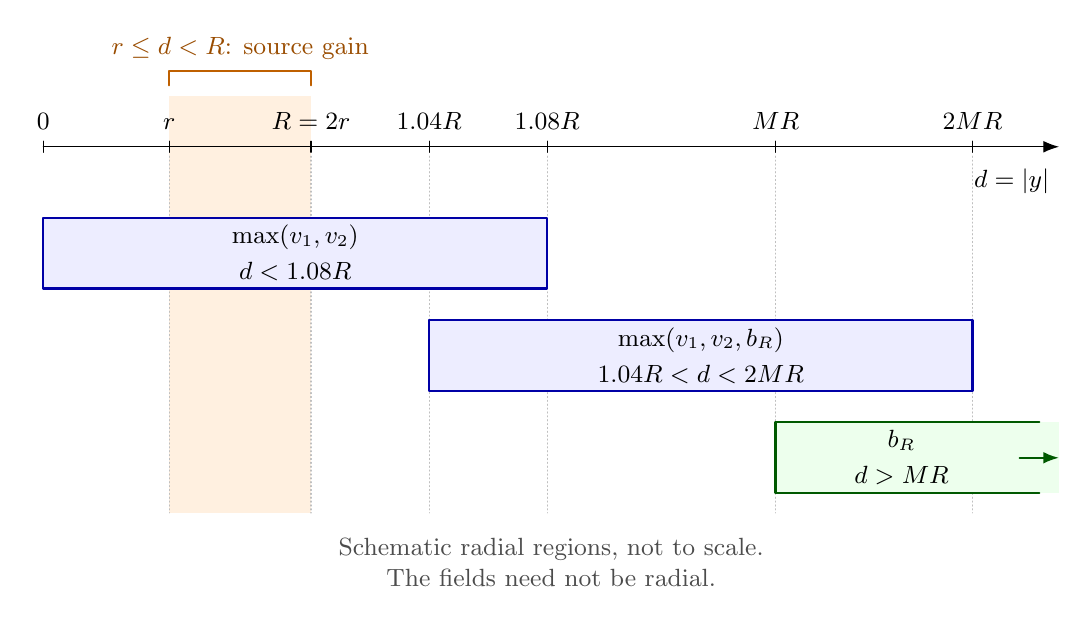
\begin{tikzpicture}[
    x=1cm,y=1cm,
    font=\fontsize{9}{11}\selectfont,
    line cap=round,
    line join=round
  ]
    \fill[orange!12] (1.6,0.65) rectangle (3.4,-4.65);
    \draw[orange!75!black,thick]
      (1.6,0.78) -- (1.6,0.96) -- (3.4,0.96) -- (3.4,0.78);
    \node[above,text=orange!60!black] at (2.5,0.99)
      {$r\le d<R$: source gain};

    \foreach \position in {1.6,3.4,4.9,6.4,9.3,11.8} {
      \draw[gray!50,densely dotted] (\position,-0.12) -- (\position,-4.65);
      \draw (\position,-0.07) -- (\position,0.07);
    }
    \draw[-{Latex[length=2mm]}] (0,0) -- (12.9,0);
    \draw (0,-0.07) -- (0,0.07);
    \node[above] at (0,0.1) {$0$};
    \node[above] at (1.6,0.1) {$r$};
    \node[above] at (3.4,0.1) {$R=2r$};
    \node[above] at (4.9,0.1) {$1.04R$};
    \node[above] at (6.4,0.1) {$1.08R$};
    \node[above] at (9.3,0.1) {$MR$};
    \node[above] at (11.8,0.1) {$2MR$};
    \node[anchor=north east] at (12.9,-0.15) {$d=|y|$};

    \filldraw[fill=blue!7,draw=blue!65!black,thick]
      (0,-0.9) rectangle (6.4,-1.8);
    \node[align=center] at (3.2,-1.35)
      {$\max(v_1,v_2)$\\[2pt]$d<1.08R$};

    \filldraw[fill=blue!7,draw=blue!65!black,thick]
      (4.9,-2.2) rectangle (11.8,-3.1);
    \node[align=center] at (8.35,-2.65)
      {$\max(v_1,v_2,b_R)$\\[2pt]$1.04R<d<2MR$};

    \fill[green!7] (9.3,-3.5) rectangle (12.9,-4.4);
    \draw[green!35!black,thick]
      (12.65,-3.5) -- (9.3,-3.5) -- (9.3,-4.4) -- (12.65,-4.4);
    \draw[green!35!black,thick,-{Latex[length=2mm]}]
      (12.4,-3.95) -- (12.9,-3.95);
    \node[align=center] at (10.9,-3.95)
      {$b_R$\\[2pt]$d>MR$};

    \node[anchor=north,align=center,text=black!70] at (6.45,-4.85)
      {Schematic radial regions, not to scale.\\
       The fields need not be radial.};
  \end{tikzpicture}
  \caption{The overlapping definitions in one continuation step from $r$ to
    $R=2r$. The shifted branches are
    $v_1=u_j-\lambda_1R^{-4}$ and
    $v_2=H'_j-\lambda_2R^{-4}$; the second branch is omitted on bad data.
    The source term changes on the shaded annulus $r\le d<R$.
    The barrier gap makes the first two definitions agree on
    $1.04R<d<1.08R$, and the caps make the last two agree on
    $MR<d<2MR$.}
  \label{fig:barrier-step}
\end{figure}


It remains to prove the weak inequality before averaging.  We do so
on open neighborhoods, to avoid differentiating across the sets
where the maximizing branch changes.  At a point in one of the
open regions in \cref{eq:barrier-open-cover}, retain the candidates
whose value is within $e_0R^{-4}$ of the maximum there.  By continuity
and finiteness, there is a neighborhood on which every discarded
candidate remains strictly below a fixed retained maximizer and
every retained candidate $v$ satisfies
\begin{equation}\label{eq:retained-branches}
 \widetilde u-v<2e_0R^{-4}.
\end{equation}
The maximum of the retained family is still $\widetilde u$ throughout
this neighborhood.  At the origin use the continuous offsets from
$V$ to make the same selection.

Every retained branch satisfies the common inequality
\begin{equation}\label{eq:common-branch-inequality}
 \Delta v\ge-4\pi\nu+4\pi\ind_{\{d<R\}}\mu_j
       -4\pi\widetilde p+\ind_{\{d\ge R\}}f(v)
\end{equation}
on this whole neighborhood.  For $v_1$, its old inequality suffices
on $d<r$, and on $d\ge R$ use $f(u)\ge f(v_1)$.
The only new source is on $r\le d<R$.  Bad data there are paid for
by \cref{eq:barrier-added-error}.  On good data $v_2$ is a candidate,
so \cref{eq:retained-branches} gives
\[
 H'_j\le u-(\lambda_1-\lambda_2-2e_0)R^{-4}.
\]
Moreover $h_l<7B/8\le d^4u\le C_{\mathrm{inv}}<h_h$.
If $4\pi\mu_j>f(u)$, the high implication of
\cref{eq:inverse-comparison}, at height $h=d^4u$, would give
\[
 H'_j\ge u-\xi d^{-4}\ge u-16\xi R^{-4},
\]
contrary to \cref{eq:barrier-parameters}.  Hence $4\pi\mu_j\le f(u)$,
which supplies the required new density.

For $v_2$ its exact identity
$\Delta v_2=-4\pi\nu+4\pi\mu_j$ suffices on $d<R$.
At a remaining point where it is retained, the lower splice or
the included barrier gives $\widetilde u\ge b_R$ and $d\le2MR$.
Consequently
\[
 d^4v_2\ge\frac{7B}{8}-2e_0(2M)^4>\frac{5B}{8}>h_l,
 \qquad d^4v_2\le C_{\mathrm{cap}}<h_h.
\]
If $4\pi\mu_j<f(v_2)$, the low implication of
\cref{eq:inverse-comparison} would imply
\[
 H'_j\le v_2+\xi d^{-4}\le v_2+\xi R^{-4}
                <v_2+\lambda_2R^{-4}=H'_j,
\]
a contradiction.  Thus $4\pi\mu_j\ge f(v_2)$ there.  The branch
$b_R$ occurs only outside $R$ and satisfies
\cref{eq:common-branch-inequality} by its subsolution property.

These comparisons concern zero-order densities almost everywhere
on the same open neighborhood, including when it crosses $d=R$.
The common reaction is $F(y,t)=\ind_{\{d\ge R\}}f(t)$.
It meets the weak maximum rule's hypotheses; near zero the common
$V$ singularity cancels and the reaction vanishes.  The rule therefore
proves \cref{eq:common-branch-inequality} for $\widetilde u$ locally.
A partition of unity proves it globally.

\paragraph{Forgetting one observation.}
Define
\[
 u_{j+1}=V+\E[\widetilde u-V\mid\mathcal F_{j+1}],
 \qquad
 p_{j+1}=\E[\widetilde p\mid\mathcal F_{j+1}].
\]
We justify the conditional integration of the weak inequality.
For a fixed system the positive minimum packet width gives
deterministic bounds for $\mu_j$, $K*\mu_j$, and its first
derivatives.  The initial truncated potential has the same bounds.
Thus the initial offsets have deterministic local Lipschitz bounds;
subtracting constants, taking finite maxima, and gluing on the fixed
open cover preserve such bounds.  Where $b_R$ is used, its offset
from $V$ is smooth and separated from the origin.  The errors remain
bounded densities supported in deterministic balls.  Conditional
integration preserves these bounds.  All fields and flags are jointly
measurable; the spatial supremum defining the initial flag can be
tested on a countable dense set.  Fubini's theorem therefore permits
conditional integration against each smooth compactly supported
test.  A countable dense family of nonnegative tests, followed by
local approximation, supplies simultaneous almost-sure weak
inequalities for all tests.

The conditional tower gives $\mu_{j+1}$ as the new inner density,
and convexity gives
\[
 \E[f(\widetilde u)\mid\mathcal F_{j+1}]
 \ge f\bigl(V+\E[\widetilde u-V\mid\mathcal F_{j+1}]\bigr).
\]
This proves the first line of \cref{eq:barrier-invariant} at $R$.
The deterministic lower and upper bounds, the equality beyond
$MR$, and the error support also pass to the conditional average.

\paragraph{Total error.}
For $r\le |y|<2r$, every master packet contributing to $\mu_j(y)$
has center in a fixed annulus comparable to $r$ and width comparable
to $r^{1+w}$.  Conditional Jensen, the packet bound, and
\cref{eq:annular-count,eq:rough-deficit} imply
\[
 \norm{\mu_j(y)}_{L^2(\Prob)}
 \le Cr^{-3-3w}\bigl(r^{-3}+\sqrt{D_0r}\bigr)
 \le Cr^{-6-3w},
\]
since $r\le s$ and $D_0\le Cs^{-7}$.  The bad band event has
probability at most $Cr^{25}$.  Cauchy--Schwarz in the data and
integration over the gain annulus therefore give
\[
 \E\int\ind_{\{\mathrm{bad}\}}\ind_{\{r\le d<R\}}\mu_j
 \le Cr^{25/2+3-6-3w}=Cr^{19/2-3w}.
\]
The sum over the geometric sequence of scales is at most
$Cs^{19/2-3w}$.  Conditional averaging preserves expected total mass.
Together with the initial error estimate this proves
\cref{eq:barrier-error-mass} and completes the induction.
\end{proof}

\section{The limiting field and its charge}\label{sec:limit}

We now prove the charge and profile assertions of
\cref{thm:priced-deficit}; \cref{prop:tf-identification} will identify
the energy coefficient.  The barrier is available at
every intermediate observation scale, before all observations are
forgotten.  This lets us select conditional fields which satisfy both
the local Thomas--Fermi equation and the small-error barrier.

\subsection{Selecting conditional data}

Take an arbitrary sequence in \cref{eq:scaling-regime}, with an
arbitrary minimizing index $n$ in each system.  By
\cref{eq:rough-deficit}, after passing to a subsequence we may suppose
\[
 q_s:=s^3(Z-n)\longrightarrow q_*.
\]
Choose integers $l\to\infty$ sufficiently slowly and a scale $j<J_*$
such that
\begin{equation}\label{eq:intermediate-scale}
 \frac1{2l}\le a_*:=\frac{r_j}{s}\le\frac1l.
\end{equation}
This is possible because $r_0/s\to0$ and the radii are dyadic.
In addition to the fixed parameters used in the barrier construction,
apply \cref{prop:inverse-comparison} at this scale with $M=l^2$, a
fixed upper height greater than $C_{\mathrm{cap}}+1$, and lower height
and tolerance sufficiently small in terms of $l$.  On its good event,
\begin{equation}\label{eq:local-tf-approximation}
 \left|\mu_j(y)-k\bigl(H'_j(y)_+\bigr)^{3/2}\right|
 \le l^{-8}|y|^{-6}
 \qquad(r_j\le|y|\le ls).
\end{equation}
Indeed, let $u=|y|^4H'_j(y)$ and
$v=(|y|^6\mu_j(y)/k)^{2/3}$.  The cap on $u$ excludes $v$ at or
above the upper height: applying the high implication at heights
approaching that endpoint would contradict the cap.  Above the
lower endpoint, the two implications at heights approaching $v$
squeeze $u$ to within the chosen tolerance of $v$.  At or below
the lower endpoint they bound $u$ above by that endpoint plus the
tolerance.  Thus $|u_+-v|\le h_l+\xi$, with both $u_+$ and $v$ in
$[0,h_h+1]$; this uses no lower bound on $u$.
Uniform continuity of $t\mapsto t^{3/2}$ on that interval proves
the assertion after choosing $h_l$ and $\xi$ sufficiently small.
The spatial range is covered because
$4Mr_j\ge2ls$.

For each fixed $l$ these are fixed parameters of
\cref{prop:inverse-comparison}; its thresholds hold eventually and
its exceptional probability tends to zero.  A slow diagonal choice
therefore makes \cref{eq:local-tf-approximation} hold outside a set
of probability tending to zero while also ensuring
\cref{eq:intermediate-scale}.

We can select data on which, in addition,
\begin{equation}\label{eq:selected-data}
 \int p_j\le1,
 \qquad
 s^3\int_{|y|>2R_0s}\mu_j(y)\,dy\le\eta_s,
 \qquad\eta_s\longrightarrow0.
\end{equation}
The first excluded probability tends to zero by
\cref{eq:barrier-error-mass}.  For the second, a master packet
centered in $|x|\le R_0s$ is contained in $|y|\le2R_0s$ for all
sufficiently far systems.  The conditional tower and
\cref{eq:exterior-cutoff} show that the expectation of its left side
tends to zero, uniformly in $j$.  Markov's inequality supplies a
deterministic threshold $\eta_s\to0$ with excluded probability
tending to zero.  These two events and the good comparison event
have positive joint probability.  Choose a point in their intersection
where all the conditional identities and barrier inequalities hold.
Only this finite-system selection is needed; every selected density
still has total mass exactly $n$.

\subsection{Compactness and the exterior boundary condition}

On the selected data, suppress the sequence index and put
\[
 F_s(x)=s^4\bigl(V-K*\mu_j\bigr)(sx),
 \qquad \rho_s(x)=s^6\mu_j(sx).
\]
Then
\[
 \Delta F_s=-4\pi Zs^3\delta_0+4\pi\rho_s,
 \qquad s^4H'_j(sx)=F_s(x)-1.
\]
The total rescaled electron mass need not be bounded.  We instead
control the screened field through its spherical mean.  Newton's
averaging identity and $\int\mu_j=n$ give
\begin{equation}\label{eq:spherical-mean}
 \overline F_s(d):=\frac1{4\pi}\int_{\mathbb S^2}F_s(d\omega)\,d\omega
 =\frac{q_s}{d}
   +\int_{|x|>d}\left(\frac1d-\frac1{|x|}\right)\rho_s(x)\,dx.
\end{equation}
In particular $\overline F_s(d)\ge q_s/d$.

On every compact annulus, \cref{prop:inverse-comparison} gives the
uniform pointwise upper bound
$F_s(x)\le1+C_{\mathrm{cap}}|x|^{-4}$ for sufficiently far systems.
Together with \cref{eq:spherical-mean} and boundedness of $q_s$, this
bounds $F_s$ in local $L^1$ away from zero: integrate
$|F_s|=2(F_s)_+-F_s$ first over spheres and then over radii.
Equation~\eqref{eq:local-tf-approximation} also bounds $\rho_s$
uniformly on these annuli.

For completeness, choose a ball whose closure avoids the origin,
and add to $F_s$ the Coulomb potential of $\rho_s$ restricted to a
slightly larger ball.  The sum is harmonic on the larger ball.
The added potential and its gradient are uniformly bounded by the
integrals of $|x-y|^{-1}$ and $|x-y|^{-2}$ against a bounded density.
Interior harmonic estimates, using the local $L^1$ bound, give
uniform bounds and equicontinuity on the smaller ball.  A diagonal
Arzel\`a--Ascoli argument now gives a subsequence converging locally
uniformly on $\R^3\setminus\{0\}$ to a field $F_\infty$.
The scaled error in \cref{eq:local-tf-approximation} tends to zero
locally uniformly, so the densities converge there to
$k((F_\infty-1)_+)^{3/2}$.  Hence
\begin{equation}\label{eq:limit-pde}
 \Delta F_\infty=4\pi k\bigl((F_\infty-1)_+\bigr)^{3/2},
 \qquad
 F_\infty(x)\le1+C_{\mathrm{cap}}|x|^{-4}.
\end{equation}
The equation holds classically off zero.  For example, bounded
local sources first give local H\"older regularity of the field;
the reaction is then locally H\"older, and interior Poisson
regularity gives the asserted conclusion.

The selected tail bound says precisely
\[
 \int_{|x|>2R_0}\rho_s(x)\,dx\longrightarrow0.
\]
Local uniform density convergence therefore makes $F_\infty$
harmonic on $|x|>2R_0$.  For $d>2R_0$, the last term of
\cref{eq:spherical-mean} is nonnegative and at most $d^{-1}$ times
this tail mass.  Consequently
\begin{equation}\label{eq:limit-exterior-mean}
 \overline F_\infty(d)=q_*/d\qquad(d>2R_0).
\end{equation}

These facts imply the uniform boundary condition
\begin{equation}\label{eq:limit-decay}
 F_\infty(x)\longrightarrow0\qquad(|x|\to\infty).
\end{equation}
Here no positivity has yet been assumed.  On large annuli rescaled
to a fixed annulus, the upper cap bounds the positive part, and
\cref{eq:limit-exterior-mean} bounds the integral of the negative
part.  Interior harmonic estimates thus give a uniform absolute
bound for $F_\infty$ throughout the exterior.  Given any sequence
$R_i\to\infty$, its dilates $F_\infty(R_i x)$ have a subsequence
converging locally on punctured space to a bounded harmonic
function, with the same absolute bound on every punctured compact
set.  Its singularity at zero is removable, and Liouville's theorem
makes it constant.  Its spherical mean is zero by
\cref{eq:limit-exterior-mean}, so the constant is zero.  If
\cref{eq:limit-decay} failed, dilating at a sequence of offending
radii and taking a convergent subsequence of the corresponding unit
directions would contradict this conclusion.  This proves uniform
decay.

\subsection{Transferring the positive barrier}

We claim that
\begin{equation}\label{eq:limit-positive-barrier}
 F_\infty(x)\ge B|x|^{-4}\qquad(x\ne0).
\end{equation}
The field in this assertion is the field without the subtracted
price.  This distinction permits the reaction comparison below.

Fix an outer radius $S>0$ and write $U_s(x)=s^4u_j(sx)$.
Inside $a_*$, the distributional inequality for $U_s$ and the
equation for $F_s$ contain the same point-nucleus and density
$\rho_s$ terms; the inequality also contains the rescaled error
from $p_j$.
Outside
$a_*$, \cref{eq:local-tf-approximation} gives, once $l>S$,
\[
 \rho_s(x)\le k\bigl((F_s(x)-1)_+\bigr)^{3/2}
                         +l^{-8}|x|^{-6}.
\]
Define the nonnegative correction potential
\begin{equation}\label{eq:barrier-correction}
 L_s=K*\left(s^6p_j(s\,\cdot)
       +l^{-8}|\cdot|^{-6}\ind_{\{a_*\le|\cdot|\le S\}}\right).
\end{equation}
Scaling \cref{eq:barrier-invariant}, subtracting the equation for
$F_s$, and using $\Delta K=-4\pi\delta_0$ gives on $B(0,S)$
\begin{equation}\label{eq:barrier-transfer-inequality}
 \Delta(U_s-F_s-L_s)
 \ge\ind_{\{|x|\ge a_*\}}\bigl[f(U_s)-f(F_s-1)\bigr].
\end{equation}
In particular, subtracting $L_s$ cancels both the accumulated
source error and the approximation error with the required sign.

Choose any
\[
 c>\left(C_{\mathrm{inv}}S^{-4}
                   -\min_{|x|=S}F_\infty(x)\right)_+.
\]
For sufficiently far systems, local uniform convergence on this
sphere, the upper bound for $U_s$, and $L_s\ge0$ give
$U_s-F_s-L_s\le c$ on the boundary.  The same inequality holds
throughout the ball.  Indeed, test
\cref{eq:barrier-transfer-inequality} with
$(U_s-F_s-L_s-c)_+$.  On its positive set,
$U_s>F_s+L_s+c>F_s-1$, so the reaction difference is nonnegative.
The test yields
\[
 \int_{B(0,S)}\left|\nabla(U_s-F_s-L_s-c)_+\right|^2\le0.
\]
It is legitimate on the full ball: the nuclear singularities in
$U_s-F_s$ cancel, the remaining offsets are continuous and locally
$H^1$, and the correction is the potential of a bounded compactly
supported density for each fixed system.  After cancellation all
right-hand sides are locally bounded, including near zero, because
the reaction term vanishes on $|x|<a_*$.  Approximation therefore
allows the compactly supported nonnegative $H^1$ test.

For each fixed $x\ne0$, $L_s(x)\to0$.  The first density in
\cref{eq:barrier-correction} has mass at most $s^3$ by
\cref{eq:selected-data} and is supported in $|x|\le a_*$.
The second has total mass at most
\[
 C l^{-8}a_*^{-3}\le C l^{-5},
\]
by \cref{eq:intermediate-scale}; its density near a fixed nonzero
evaluation point is $O_x(l^{-8})$.  Splitting its potential integral
into a small ball around that point and its complement proves the
claim.  Finally, for fixed $0<|x|<S$ and sufficiently far systems,
\[
 U_s(x)\ge B|x|^{-4}\left(1-\frac{a_*}{8|x|}\right).
\]
Pass to the limit in $U_s\le F_s+L_s+c$, then decrease $c$ to its
permitted endpoint.  Letting $S\to\infty$ and using
\cref{eq:limit-decay} proves \cref{eq:limit-positive-barrier}.

\subsection{The singular profile and uniqueness}

The dilation argument below is a direct form of the Sommerfeld comparison
principle. The homogeneous zero-price profiles are covered by
\cite[Lemma~4.4 and Remark~4.5]{Solovej2003}, including nonspherical fields.
Here dilation removes the unit price near the singularity; a separate
comparison then proves uniqueness for the priced equation.

\begin{lemma}[Unique decaying singular profile]\label{lem:singular-profile}
There is at most one classical solution $F$ of
\[
 \Delta F=4\pi k\bigl((F-1)_+\bigr)^{3/2}
       \quad\text{on }\R^3\setminus\{0\}
\]
which tends uniformly to zero at infinity and satisfies
$c|x|^{-4}\le F(x)\le C|x|^{-4}$ near zero for some $c,C>0$.
Every such solution has the uniform singular asymptotic
\begin{equation}\label{eq:sommerfeld-coefficient}
 |x|^4F(x)\longrightarrow
 A_{\mathrm S}:=\left(\frac{12}{4\pi k}\right)^2
       \qquad(|x|\downarrow0).
\end{equation}
If a solution exists, it is radial.
\end{lemma}

\begin{proof}
Let $a$ and $b$ be the lower and upper limits of $|x|^4F(x)$ at zero;
the hypotheses give $0<a\le b<\infty$.  Choose points approaching
the upper limit and put $t$ equal to their radii.  The dilates
$u_t(x)=t^4F(tx)$ satisfy
\[
 \Delta u_t=4\pi k\bigl((u_t-t^4)_+\bigr)^{3/2}.
\]
They are bounded above and below by positive multiples of $|x|^{-4}$
on compact annuli.  The local potential and harmonic compactness
argument used above supplies a subsequential classical limit $u$
with $\Delta u=4\pi k u^{3/2}$.  The definition of $b$ gives
$u(x)\le b|x|^{-4}$ for every $x\ne0$.  After taking a subsequence
of the unit directions, equality holds at a unit point.  The
difference $u-b|x|^{-4}$ has a local maximum there, so
\[
 4\pi k b^{3/2}\le12b.
\]
The analogous dilation at points approaching the lower limit touches
$a|x|^{-4}$ from above at a unit point and gives
$4\pi k a^{3/2}\ge12a$.  Since both constants are positive,
\[
 b\le\left(\frac{12}{4\pi k}\right)^2\le a.
\]
This proves \cref{eq:sommerfeld-coefficient}.  The contact argument
does not assume radiality.

Let $F_1,F_2$ be two such solutions.  For $\alpha>1$ and $\delta>0$,
the function $G=\alpha F_1+\delta$ is an upper comparison function:
\[
 \Delta G=\alpha\,4\pi k\bigl((F_1-1)_+\bigr)^{3/2}
       \le4\pi k\bigl((G-1)_+\bigr)^{3/2}.
\]
If $F_1\le1$ the inequality is immediate; otherwise use
$G-1\ge\alpha(F_1-1)$ and $\alpha^{3/2}\ge\alpha$.
The common asymptotic coefficient makes $G$ dominate $F_2$ on all
sufficiently small spheres.  Uniform decay and $\delta>0$ give
domination on all sufficiently large spheres.  On the intervening
annulus, testing with $(F_2-G)_+$ and using the nondecreasing
reaction proves $F_2\le G$.  Thus this inequality holds everywhere.
Let $\delta\downarrow0$ and $\alpha\downarrow1$, and interchange
the two solutions to obtain equality.  Rotations preserve the
equation and both boundary conditions, so uniqueness also gives
radiality.
\end{proof}

\begin{proof}[The charge assertion of \cref{thm:priced-deficit}]
The field $F_\infty$ constructed above satisfies the hypotheses of
\cref{lem:singular-profile}, by
\cref{eq:limit-pde,eq:limit-decay,eq:limit-positive-barrier}.
In particular a solution exists, is unique, and is radial.
Its exterior mean determines $q_*$ uniquely by
\cref{eq:limit-exterior-mean}.  Moreover, at any fixed $d>2R_0$,
\[
 \frac{q_*}{d}=\overline F_\infty(d)\ge Bd^{-4}>0.
\]
Denote this uniquely determined positive number by $q$.
The reaction density vanishes beyond $2R_0$, and radiality together
with \cref{eq:limit-exterior-mean} gives $F_\infty(x)=q/|x|$ there.

Every sequence of systems and every choice of minimizing indices
has bounded scaled deficits by \cref{eq:rough-deficit}.  From any
subsequence on which these deficits converge, the preceding
construction produces the same unique profile and hence the same
limit $q$.  Therefore all scaled deficits converge to $q$:
\[
 s^3(Z-n)\longrightarrow q>0
 \qquad\text{along }\cref{eq:scaling-regime}.
\]
The argument allowed an arbitrary minimizing index at every stage,
as required.  The remaining coefficient identity in
\cref{thm:priced-deficit} is proved in \cref{prop:tf-identification}.
\end{proof}

\section{Fixed particle numbers and the Thomas--Fermi coefficient}
\label{sec:fixed-sectors}

We first recover fixed-sector energy differences from the priced deficit
proved in \cref{sec:limit}.  This step uses monotonicity of the sector
energies, without requiring convexity or requiring every sector to minimize
at some price.  The priced minimum is concave in the price, and its
minimizing sectors bound its secant slopes even when the minimizing sector
changes.  Integrating the deficit law therefore determines the energy at
those sectors; monotonicity then brackets the desired particle number.
We identify the coefficient by the corresponding Thomas--Fermi calculation.

\subsection{Integrating the price and bracketing the sector}

\begin{proposition}\label{prop:fixed-sector-limit}
Let $q$ be the deficit coefficient in \cref{thm:priced-deficit}.  For every
sequence of integers $Z>m\ge1$ such that $m\to\infty$ and $Z/m\to\infty$,
\begin{equation}\label{eq:fixed-sector-limit}
 \frac{E_Z(Z-m)-E_Z(Z)}{m^{7/3}}
       \longrightarrow\frac37q^{-4/3}.
\end{equation}
\end{proposition}

\begin{proof}
Fix such a sequence.  At each fixed $t>0$, choose any index $n_t$ minimizing
$E_n+tm^{4/3}n$, and put
\[
 d_{Z,m}(t)=\frac{Z-n_t}{m},\qquad
 G_{Z,m}(t)=m^{-7/3}
       \bigl[P(tm^{4/3})-tm^{4/3}Z-E_Z(Z)\bigr].
\]
The choice $s=t^{-1/4}m^{-1/3}$ satisfies
\cref{eq:scaling-regime}, since $Zs^3=t^{-3/4}Z/m\to\infty$.
The deficit assertion of \cref{thm:priced-deficit} therefore gives
\begin{equation}\label{eq:priced-scaled-deficit}
 d_{Z,m}(t)\longrightarrow qt^{3/4}
 \qquad\text{for every fixed }t>0,
\end{equation}
for every choice of the minimizing indices.

For $0<v<t$, the minimizers at the two endpoint prices give
\begin{equation}\label{eq:quantum-secants}
 -d_{Z,m}(t)\le
       \frac{G_{Z,m}(t)-G_{Z,m}(v)}{t-v}
       \le-d_{Z,m}(v).
\end{equation}
Indeed, evaluating the objective at $n_v$ gives the upper inequality,
and evaluating the objective at $n_t$ at price $v$ gives the lower one.
These inequalities do not require differentiability at a price with more
than one minimizing sector.

Take a fixed partition $v=t_0<t_1<\cdots<t_r=t$.  Summing
\cref{eq:quantum-secants} bounds $G_{Z,m}(t)-G_{Z,m}(v)$ by the two endpoint
Riemann sums for the negative deficits.  First use
\cref{eq:priced-scaled-deficit} at the finitely many partition points, and
then refine the partition.  Since $qt^{3/4}$ is continuous, this proves
\begin{equation}\label{eq:quantum-price-increments}
 G_{Z,m}(t)-G_{Z,m}(v)
       \longrightarrow-\frac47q\bigl(t^{7/4}-v^{7/4}\bigr).
\end{equation}
The behavior at zero price fixes the integration constant.  The neutral
sector is a competitor, whereas $E_{n_v}\ge E\ge E_Z(Z)-C$ by
\cref{eq:neutral-offset}; hence
\begin{equation}\label{eq:quantum-zero-endpoint}
 -Cm^{-7/3}-v\,d_{Z,m}(v)\le G_{Z,m}(v)\le0.
\end{equation}
For every fixed $v>0$ this gives
$\limsup|G_{Z,m}(v)|\le qv^{7/4}$.  Combining it with
\cref{eq:quantum-price-increments} and then sending $v\downarrow0$ yields
\begin{equation}\label{eq:quantum-price-energy}
 G_{Z,m}(t)\longrightarrow-\frac47qt^{7/4},\qquad
 \frac{E_{n_t}-E_Z(Z)}{m^{7/3}}
       =G_{Z,m}(t)+t\,d_{Z,m}(t)
       \longrightarrow\frac37qt^{7/4}.
\end{equation}
Thus no assertion about the convergence of the priced minimizers as
$t\downarrow0$ was needed.

Choose fixed prices
\[
 0<t_-<q^{-4/3}<t_+.
\]
By \cref{eq:priced-scaled-deficit}, their deficits are eventually smaller
and larger than $m$, respectively.  Thus
$n_{t_-}>Z-m>n_{t_+}$.  Monotonicity of the sector energies gives
\[
 E_{n_{t_-}}-E_Z(Z)
       \le E_Z(Z-m)-E_Z(Z)
       \le E_{n_{t_+}}-E_Z(Z).
\]
Apply \cref{eq:quantum-price-energy} and let both prices approach
$q^{-4/3}$.  The two bounds converge to
$\frac37q(q^{-4/3})^{7/4}=\frac37q^{-4/3}$, proving
\cref{eq:fixed-sector-limit}.
\end{proof}

\subsection{The same charge in Thomas--Fermi theory}

The classical weak-ionization law was established by B\'enilan and Brezis
\cite[Section~6, Corollary~5]{BenilanBrezis2004}, following the bounds and
chemical-potential integration argument of Lieb and Simon
\cite[Theorems~IV.11--IV.12]{LiebSimon1977}.
We give the argument in the present normalization to identify its
coefficient with the charge obtained from the conditional quantum limit.

We allow real nuclear charges and real electron masses in this subsection.
For clarity, the admissible finite-mass class can be written as
\[
 \mathcal X=\{\rho\ge0:\rho\in L^1(\R^3)\cap L^{5/3}(\R^3)\}.
\]
All terms of $\mathcal T_Z$ are finite on this class.  For the direct term,
interpolation gives $\rho\in L^{6/5}$, and the Sobolev inequality gives the
embedding $L^{6/5}\subset(\dot H^1)^*$ and the finite Coulomb energy.
For the nuclear term, use $|x|^{-1}\in L^{5/2}_{\mathrm{loc}}$ near zero
and the finite mass away from zero.  Thus this is precisely the finite-mass
class in the definition of $E_Z^{\TF}(M)$.

\begin{proposition}\label{prop:tf-identification}
With the two-spin coefficient $T$ fixed above,
\begin{equation}\label{eq:tf-unit-deficit}
 \lim_{Z\to\infty}
       \bigl[E_Z^{\TF}(Z-1)-E_Z^{\TF}(Z)\bigr]
       =\frac37q^{-4/3}.
\end{equation}
The limit holds through real charges $Z>1$.  Consequently
\cref{eq:tf-constant} holds for every fixed real $m>0$, with
\[
 a_{\TF}=\frac37q^{-4/3}>0.
\]
\end{proposition}

\begin{proof}
We identify the charge in the unit-price Thomas--Fermi problem, then
integrate in the price and use the exact density scaling.

\paragraph{Monotonicity in the electron mass.}
The energy $E_Z^{\TF}(M)$ is nonincreasing in $M$.  To see this without an
attainment assumption, truncate any admissible density of mass $M_1$ to a
large ball.  The kinetic, nuclear, and direct terms converge to the
original ones.  If $M_2\ge M_1$, place the missing mass in a nonnegative
smooth packet of diameter proportional to $R$, centered at distance
$R^2$ from that ball.  For a packet of mass $a$ and this spatial scale,
its kinetic and direct energies are $O(a^{5/3}R^{-2})$ and
$O(a^2R^{-1})$.  Its nuclear term and its interaction with the fixed
truncated density tend to zero as $R\to\infty$.  The mass $a$ stays
bounded during this construction.  Taking first $R\to\infty$, then the
truncation radius to infinity, and then the original energy down to its
infimum proves monotonicity.  The same argument shows that imposing mass
exactly $M$ or at most $M$ gives the same infimum.

\paragraph{The zero-price minimizer is neutral.}
Apply \cite[\FTFPair]{Foundation} to the single positive point
source $Z\delta_0$.  Their unconstrained problem on
$L^{5/3}\cap(\dot H^1)^*$ has a unique minimizer $\rho_0$, with finite
mass at most $2Z$.  Its field $\phi_0=V-K*\rho_0$ satisfies
\begin{equation}\label{eq:tf-neutral-field}
 \rho_0=k(\phi_0)_+^{3/2},\qquad
 \Delta\phi_0=-4\pi Z\delta_0+4\pi\rho_0,\qquad
 c\min\left(\frac Z{|x|},|x|^{-4}\right)
       \le\phi_0(x)\le C|x|^{-4}.
\end{equation}
The cited lemmas supply the lower bound, finite mass, and decay at infinity.
For completeness, the upper bound is independent of $Z$: on a ball
$B(x,R)$ with $R=|x|/2$, compare $\phi_0$ with
\[
 v(y)=\frac{C R^4}{(R^2-|y-x|^2)^4}.
\]
For sufficiently large universal $C$, direct differentiation gives
$\Delta v\le4\pi k v^{3/2}$.  The function diverges at the boundary,
and the positive-part comparison for
$\Delta\phi_0=4\pi k\phi_0^{3/2}$ in this ball gives
$\phi_0(x)\le CR^{-4}$, as asserted.

Uniqueness makes $\rho_0$ and $\phi_0$ radial.  Newton's spherical-mean
identity and finite mass give
\[
 Z-\int\rho_0=\lim_{d\to\infty}d\phi_0(d)=0,
\]
where the last equality follows from \cref{eq:tf-neutral-field}.
Therefore $\int\rho_0=Z$ and
\begin{equation}\label{eq:tf-neutral-minimum}
 E_Z^{\TF}(Z)=\min_{\rho\in\mathcal X}\mathcal T_Z(\rho).
\end{equation}
There is no discrepancy between the variational classes here: every
finite-mass admissible density belongs to the cited Coulomb-dual class,
and the cited minimizer has finite mass and finite energy terms, hence
belongs to $\mathcal X$.

\paragraph{The unit-price minimizer.}
Minimize $\mathcal T_Z(\rho)+\int\rho$ over $\mathcal X$.
Removing density from the region $V\le1$ cannot increase this functional:
the kinetic term, the contribution $\int(1-V)\rho$ there, and all removed
direct interactions are nonnegative.  We may therefore restrict to the
ball $B(0,Z)$.  Since $V\in L^{5/2}(B(0,Z))$, coercivity and weak lower
semicontinuity in $L^{5/3}$ give a minimizer, and strict convexity of the
kinetic term gives uniqueness.  Denote it by $\rho_Z$ and put
$\phi_Z=V-K*\rho_Z$.  Nonnegative variations, followed by two-sided
multiplicative variations on the positive density, give
\begin{equation}\label{eq:tf-priced-euler}
 \rho_Z=k\bigl((\phi_Z-1)_+\bigr)^{3/2},\qquad
 \Delta\phi_Z=-4\pi Z\delta_0+4\pi\rho_Z.
\end{equation}
This holds globally: outside $B(0,Z)$ one has $\phi_Z\le V\le1$.
The minimizer and its field are radial by uniqueness.

The following comparison is the unit-price case of the classical
chemical-potential comparison \cite[Lemma~5.1]{Solovej2003}; we include
the short maximum-principle proof. The two fields satisfy
\begin{equation}\label{eq:tf-price-comparison}
 \phi_0\le\phi_Z\le\phi_0+1.
\end{equation}
For the first inequality, on a positive set of
$\phi_0-\phi_Z-\eta$, with $\eta>0$, the difference of the two reaction
terms in \cref{eq:tf-neutral-field,eq:tf-priced-euler} is nonnegative.
Testing with that positive part gives a nonpositive squared-gradient
bound and hence a zero test.  The test is compactly supported because
both potentials tend to zero at infinity.  For the second inequality,
$\phi_0+1$ solves the same unit-price equation away from the common
point source, and the same comparison applies.  At the origin the point
singularities cancel; the remaining potentials are continuous and locally
$H^1$, with locally $L^{5/3}$ source densities.  Thus the compact tests
are justified by $H^1$ approximation.  Let $\eta\downarrow0$ to obtain
\cref{eq:tf-price-comparison}.  The continuity and decay used here hold for
Coulomb potentials of finite $L^1\cap L^{5/3}$ densities, as also proved
in \cite[\FTFExistence]{Foundation}.

Write
\[
 Q_Z=Z-\int\rho_Z.
\]
By \cref{eq:tf-price-comparison}, $\phi_Z\ge0$ and
$\rho_Z\le k\phi_0^{3/2}\le C|x|^{-6}$.  Newton's identity reads
\begin{equation}\label{eq:tf-priced-mean}
 \phi_Z(d)=\frac{Q_Z}{d}
       +\int_{|y|>d}\left(\frac1d-\frac1{|y|}\right)\rho_Z(y)\,dy.
\end{equation}
Finite mass gives $Q_Z=\lim_{d\to\infty}d\phi_Z(d)\ge0$.
At $d=1$, the nonnegative second term and
\cref{eq:tf-price-comparison} give $Q_Z\le\phi_Z(1)\le C+1$.
Using the exterior integral of $C|y|^{-6}$ in
\cref{eq:tf-priced-mean}, we conclude
\begin{equation}\label{eq:tf-uniform-exterior}
 0\le\phi_Z(d)\le\frac C d+Cd^{-4}.
\end{equation}
Choose a fixed sufficiently large $R$.  Then $\phi_Z<1$ on $d>R$ for
every $Z$, so \cref{eq:tf-priced-euler} implies $\rho_Z=0$ there and
$\phi_Z(d)=Q_Z/d$.

\paragraph{Identification of the limiting charge.}
Let $Z\to\infty$ through real values.  On every compact annulus,
\cref{eq:tf-neutral-field,eq:tf-price-comparison} bound $\phi_Z$ above
and below, and \cref{eq:tf-priced-euler} bounds its source.  Local Poisson
estimates give a locally uniformly convergent subsequence.  Its limit
$\phi_\infty$ satisfies \cref{eq:limit-pde} and
\[
 c|x|^{-4}\le\phi_\infty(x)\le1+C|x|^{-4}.
\]
The uniform estimate \cref{eq:tf-uniform-exterior} gives decay at infinity.
By the uniqueness in \cref{lem:singular-profile}, this is the same field
constructed in \cref{sec:limit}.  Its exterior charge is $q$.  At any
fixed radius beyond both exterior supports,
$Q_Z=d\phi_Z(d)\to d\phi_\infty(d)=q$.  Uniqueness of the subsequential
limit therefore proves
\begin{equation}\label{eq:tf-unit-charge}
 Q_Z\longrightarrow q\qquad(Z\longrightarrow\infty).
\end{equation}
The use of real charges is permitted by the arbitrary-positive-point-source
hypotheses of \cite[\FTFPair]{Foundation}.

\paragraph{Other prices and their energies.}
For $t>0$, let $\rho_{Z,t}$ minimize
$\mathcal T_Z(\rho)+t\int\rho$, and write
$Q_Z(t)=Z-\int\rho_{Z,t}$.  Existence and uniqueness follow as above,
now restricting to $B(0,Z/t)$.  With $b=t^{-1/4}$, the transformation
\[
 \widetilde\rho(x)=b^6\rho_{Z,t}(bx),\qquad
 \widetilde\phi(x)=b^4\bigl(V-K*\rho_{Z,t}\bigr)(bx)
\]
gives the unit-price minimizer and field at nuclear charge $b^3Z$.
Indeed, the transformed functional is exactly
\[
 \mathcal T_{b^3Z}(\widetilde\rho)+\int\widetilde\rho
       =b^7\left(\mathcal T_Z(\rho_{Z,t})
                                      +t\int\rho_{Z,t}\right),
\]
and this transformation is a bijection of admissible densities.
Its mass is multiplied by $b^3$, so
\begin{equation}\label{eq:tf-price-scaling}
 Q_Z(t)=t^{3/4}Q_{t^{-3/4}Z}
       \longrightarrow qt^{3/4}
       \qquad(t>0\text{ fixed}).
\end{equation}

Define
\[
 \Pi_Z(t)=\min_{\rho\in\mathcal X}
                  \left(\mathcal T_Z(\rho)+t\int\rho\right),\qquad
 G_Z^{\TF}(t)=\Pi_Z(t)-tZ-E_Z^{\TF}(Z).
\]
The endpoint-minimizer comparisons give, for $0<v<t$,
\[
 -Q_Z(t)\le
      \frac{G_Z^{\TF}(t)-G_Z^{\TF}(v)}{t-v}
      \le-Q_Z(v).
\]
The exact zero-price identity \cref{eq:tf-neutral-minimum} gives
\[
 -vQ_Z(v)\le G_Z^{\TF}(v)\le0.
\]
Consequently the same fixed-partition integration and then $v\downarrow0$
argument used in \cref{eq:quantum-price-increments,eq:quantum-zero-endpoint}
gives
\begin{equation}\label{eq:tf-priced-energy}
 G_Z^{\TF}(t)\longrightarrow-\frac47qt^{7/4},\qquad
 \mathcal T_Z(\rho_{Z,t})-E_Z^{\TF}(Z)
       \longrightarrow\frac37qt^{7/4}.
\end{equation}
Each priced minimizer is also a minimizer at its own mass: an improvement
at that mass would improve the priced objective.  For fixed
$t_-<q^{-4/3}<t_+$, \cref{eq:tf-price-scaling} places these two masses on
opposite sides of $Z-1$ for all large $Z$.  The mass monotonicity proved
above and \cref{eq:tf-priced-energy}, followed by
$t_-,t_+\to q^{-4/3}$, give \cref{eq:tf-unit-deficit}.

\paragraph{Every fixed removed mass.}
For $m>0$ the density scaling
\[
 \rho(x)=m^2\sigma(m^{1/3}x)
\]
multiplies the mass by $m$ and satisfies
$\mathcal T_Z(\rho)=m^{7/3}\mathcal T_{Z/m}(\sigma)$.
It is a bijection between the corresponding admissible classes.  Hence
\begin{equation}\label{eq:tf-mass-scaling}
 E_Z^{\TF}(N)=m^{7/3}E_{Z/m}^{\TF}(N/m),\qquad
 I_m^{\TF}(Z)=m^{7/3}I_1^{\TF}(Z/m).
\end{equation}
For fixed $m>0$, the real charge $Z/m$ tends to infinity with $Z$.
Applying \cref{eq:tf-unit-deficit} proves \cref{eq:tf-constant} and the
claimed value of $a_{\TF}$.  This also completes the coefficient assertion
of \cref{thm:priced-deficit}.
\end{proof}

\subsection{The specified order of limits}

\begin{proof}[Completion of the proof of \cref{thm:main}]
The joint conclusion \cref{eq:joint-limit} follows from
\cref{prop:fixed-sector-limit,prop:tf-identification}.
To deduce the iterated limits, suppose first that, along unbounded integers
$m_j$, the normalized inner upper limit exceeds $a_{\TF}$ by a fixed
$\eta>0$.  By the definition of a limsup, for each $j$ one may choose an
arbitrarily large integer $Z_j>m_j$, in particular $Z_j/m_j\ge j$, with
\[
 \frac{I_{m_j}(Z_j)}{m_j^{7/3}}>a_{\TF}+\eta/2.
\]
This contradicts \cref{eq:joint-limit}.  The same selection applies if
these inner upper limits are infinite.  Likewise, a normalized inner lower
limit less than $a_{\TF}-\eta$ along unbounded $m_j$ allows choosing
$Z_j/m_j\ge j$ with normalized energies below $a_{\TF}-\eta/2$, again a
contradiction.  Therefore
\[
 \limsup_{m\to\infty}
       \frac{\limsup_{Z\to\infty}I_m(Z)}{m^{7/3}}\le a_{\TF},
 \qquad
 \liminf_{m\to\infty}
       \frac{\liminf_{Z\to\infty}I_m(Z)}{m^{7/3}}\ge a_{\TF}.
\]
Since the inner lower limit never exceeds the inner upper limit, both
outer limits exist and equal $a_{\TF}$.  The construction always chooses
$Z$ only after $m$ is fixed; no convergence in $Z$ at a fixed $m$ has been
assumed.
\end{proof}

\begingroup
\small
\raggedright
\phantomsection
\addcontentsline{toc}{section}{References}
\bibliographystyle{plain}
\bibliography{references}
\endgroup
\end{document}
